\chapter{Method}
\label{Method}
The flow diagram in figure \ref{fig:network} outlines the IoT test bed constructed for this project. IoT devices pull power from the outlets through the smart switches, which log the power usage, and the WAP will query the smart switches for that data and pushes it to an AWS (Amazon Web Services)\cite{rds} MySql\cite{mysql} database as an entry in the `power' table.

The wireless net provided through the WAP intercepts network packets of devices connected to it (IoT devices in tesbed), parses them into power and network entries, and pushes them to the database. Finally, for analysis, a python script called realTimeGrapher.py pulls from the database and graphs this data in real time or from set intervals in the past.

Section \ref{Physical Layout and Setup} discuss what devices we used, the set up of each device, and the physical layout of the IoT test bed. Section \ref{software} will go over the software part of the IoT test bed. It covers the usage flow of this test bed and what was done to obtain results for analysis.

\begin{figure}[H]
    \centering
    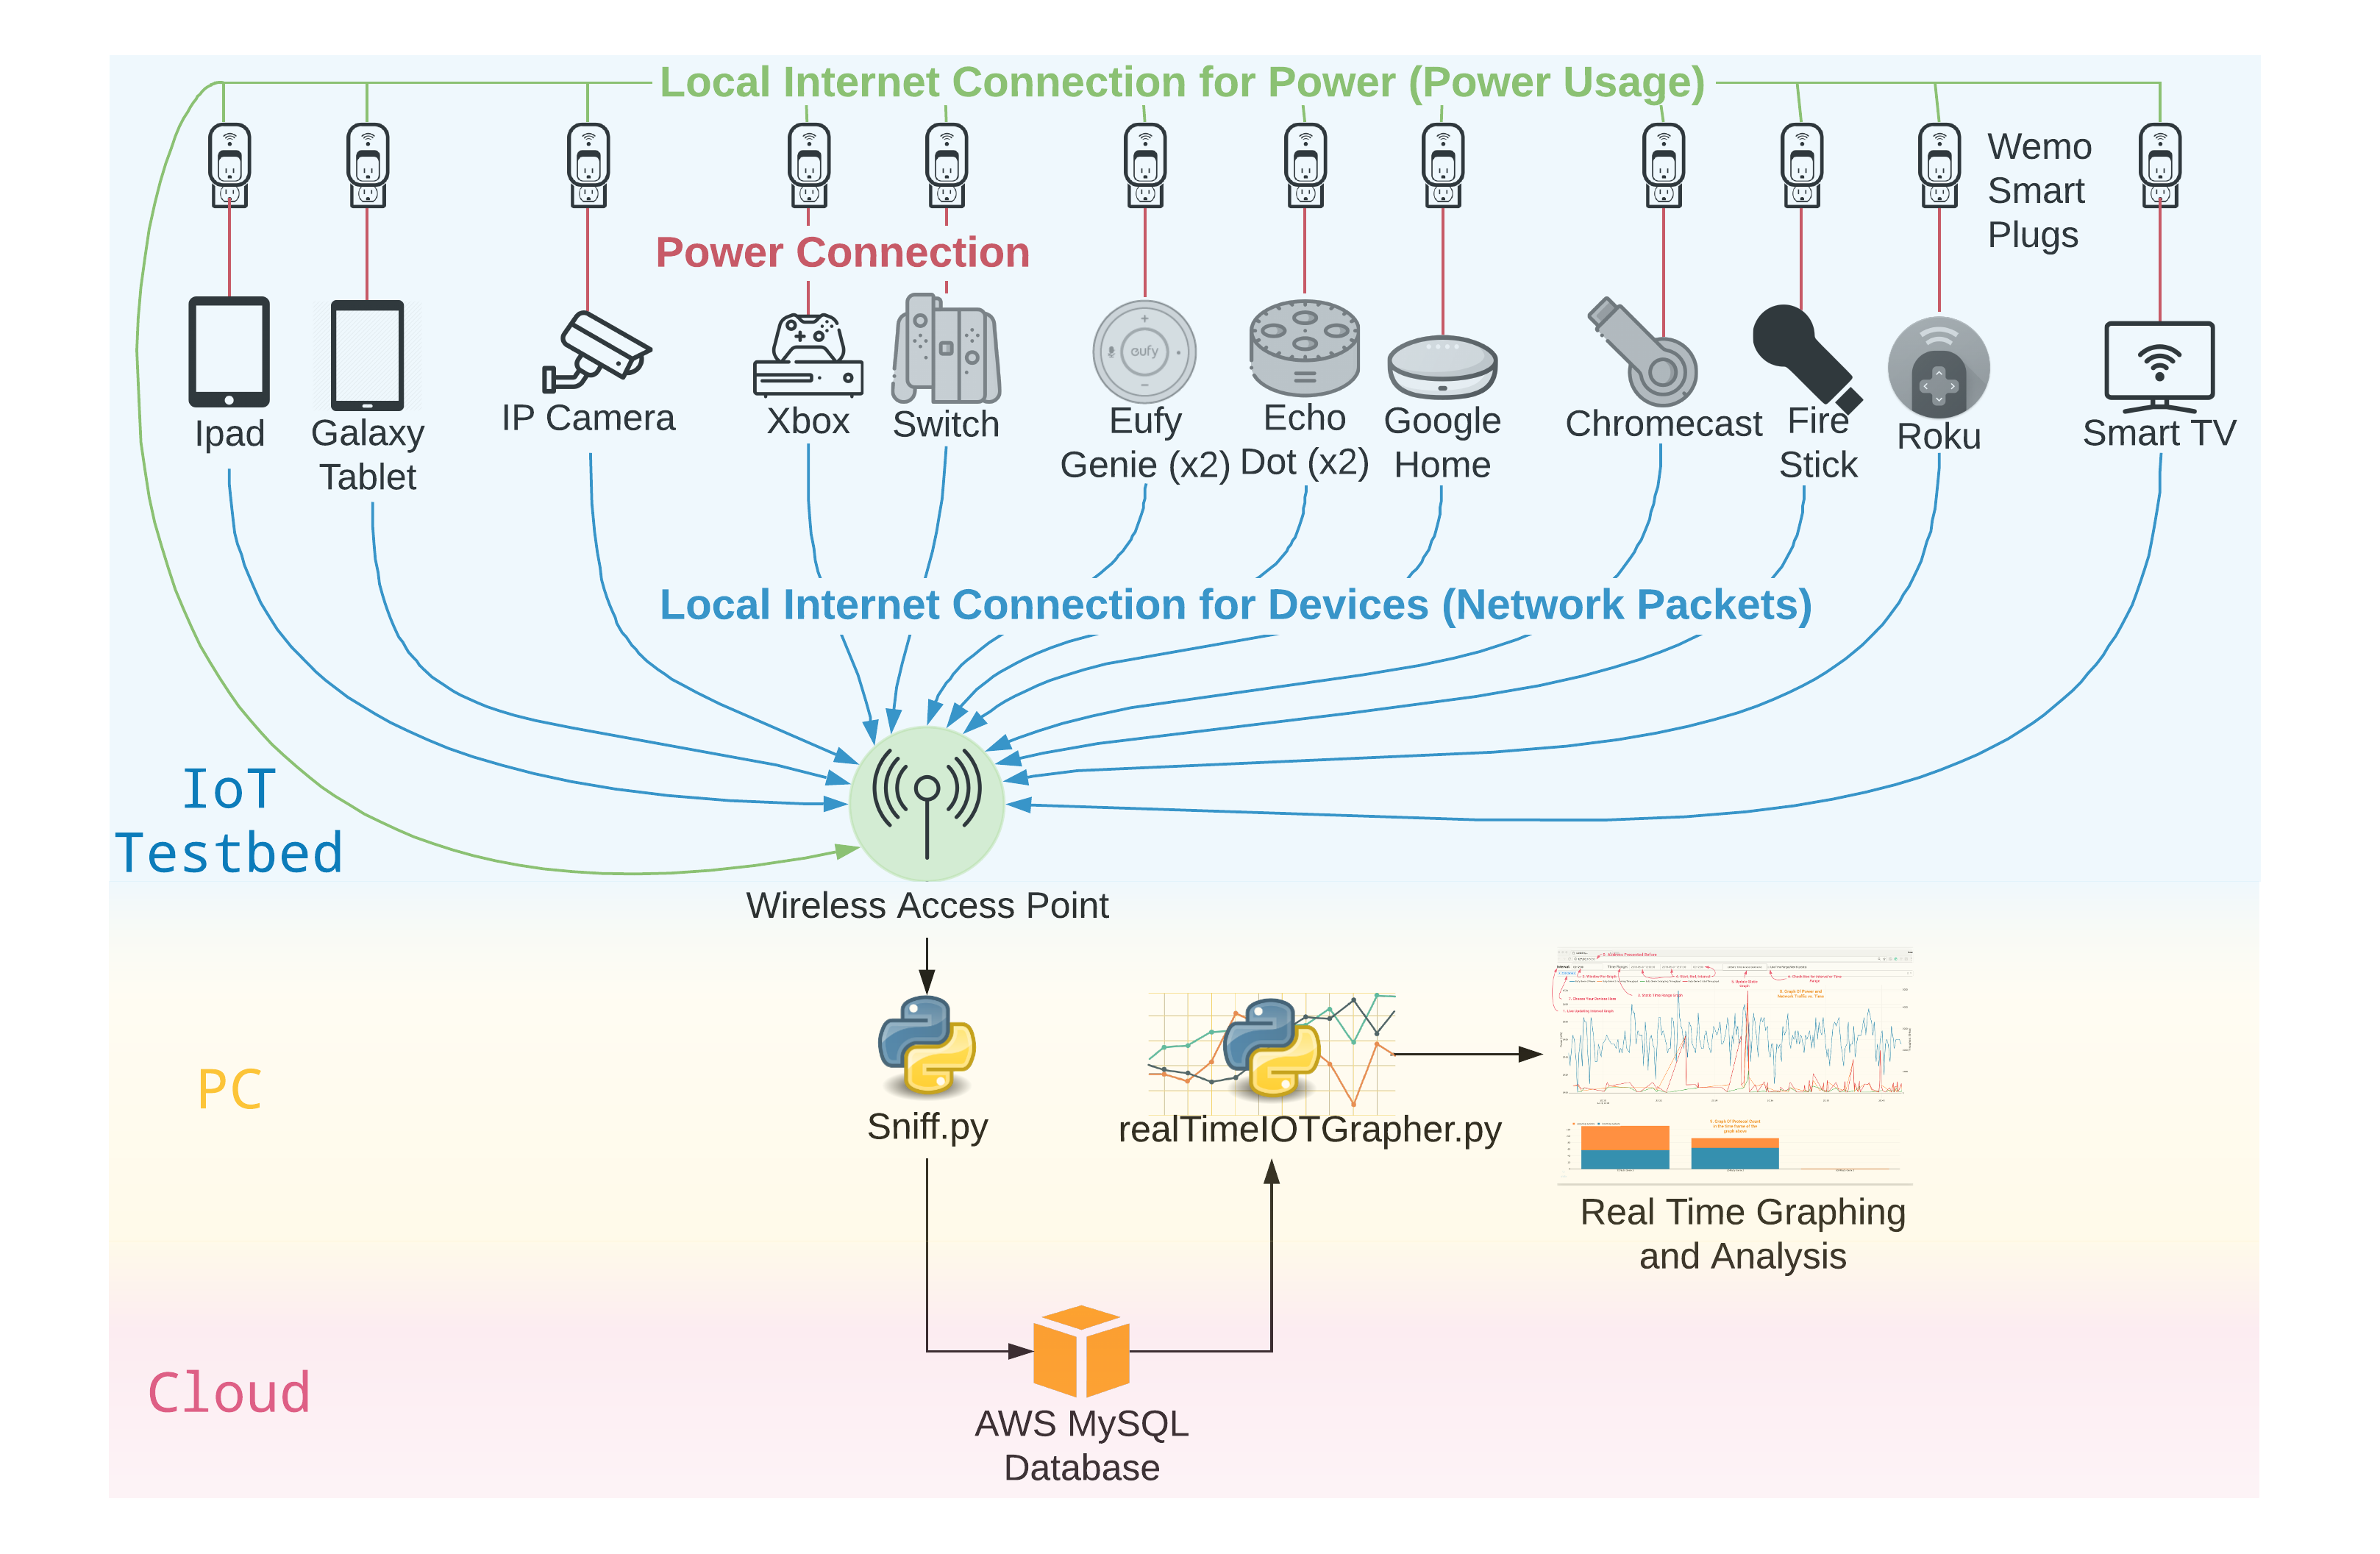
\includegraphics[width=1.0\textwidth]{networkDiagram}
    \caption{Network Diagram}
    \label{fig:network}
\end{figure}

\begin{figure}[H]
    \centering
    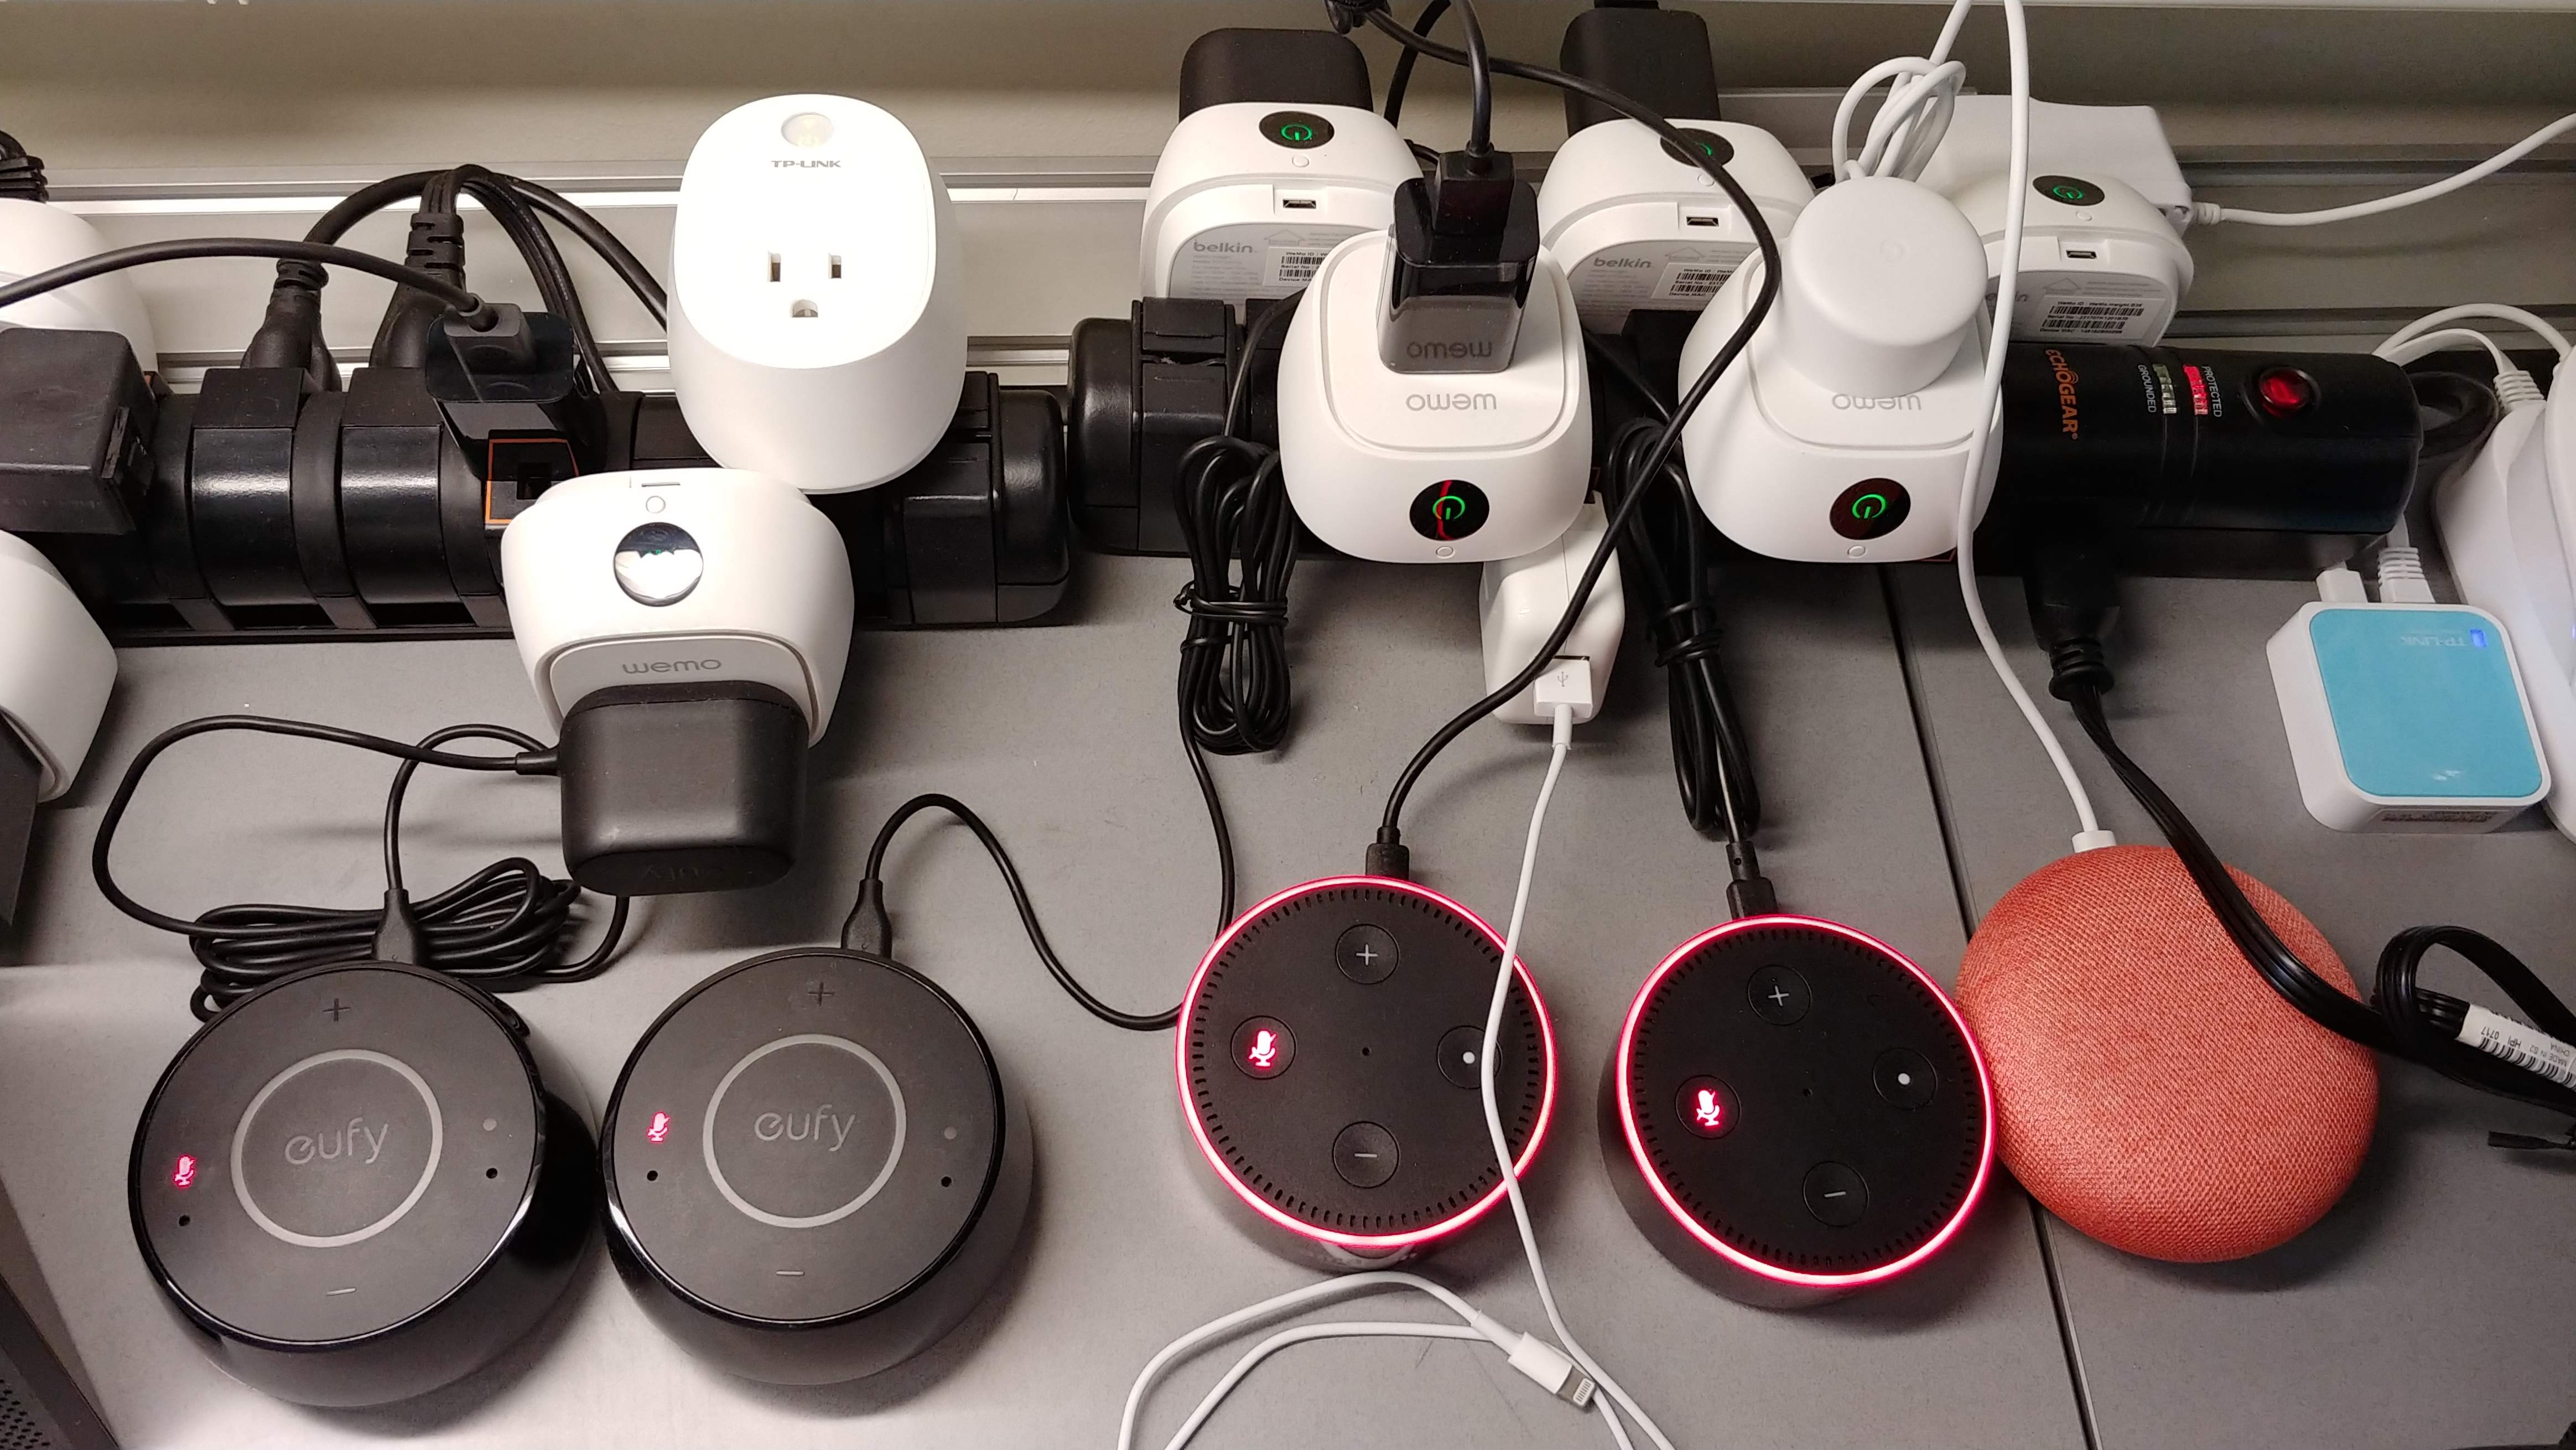
\includegraphics[width=1\textwidth]{wemos}
    \caption{Smart Speakers Connected to Wemo Insight Switches}
    \label{fig:wemo}
\end{figure}

\begin{figure}[H]
    \centering
    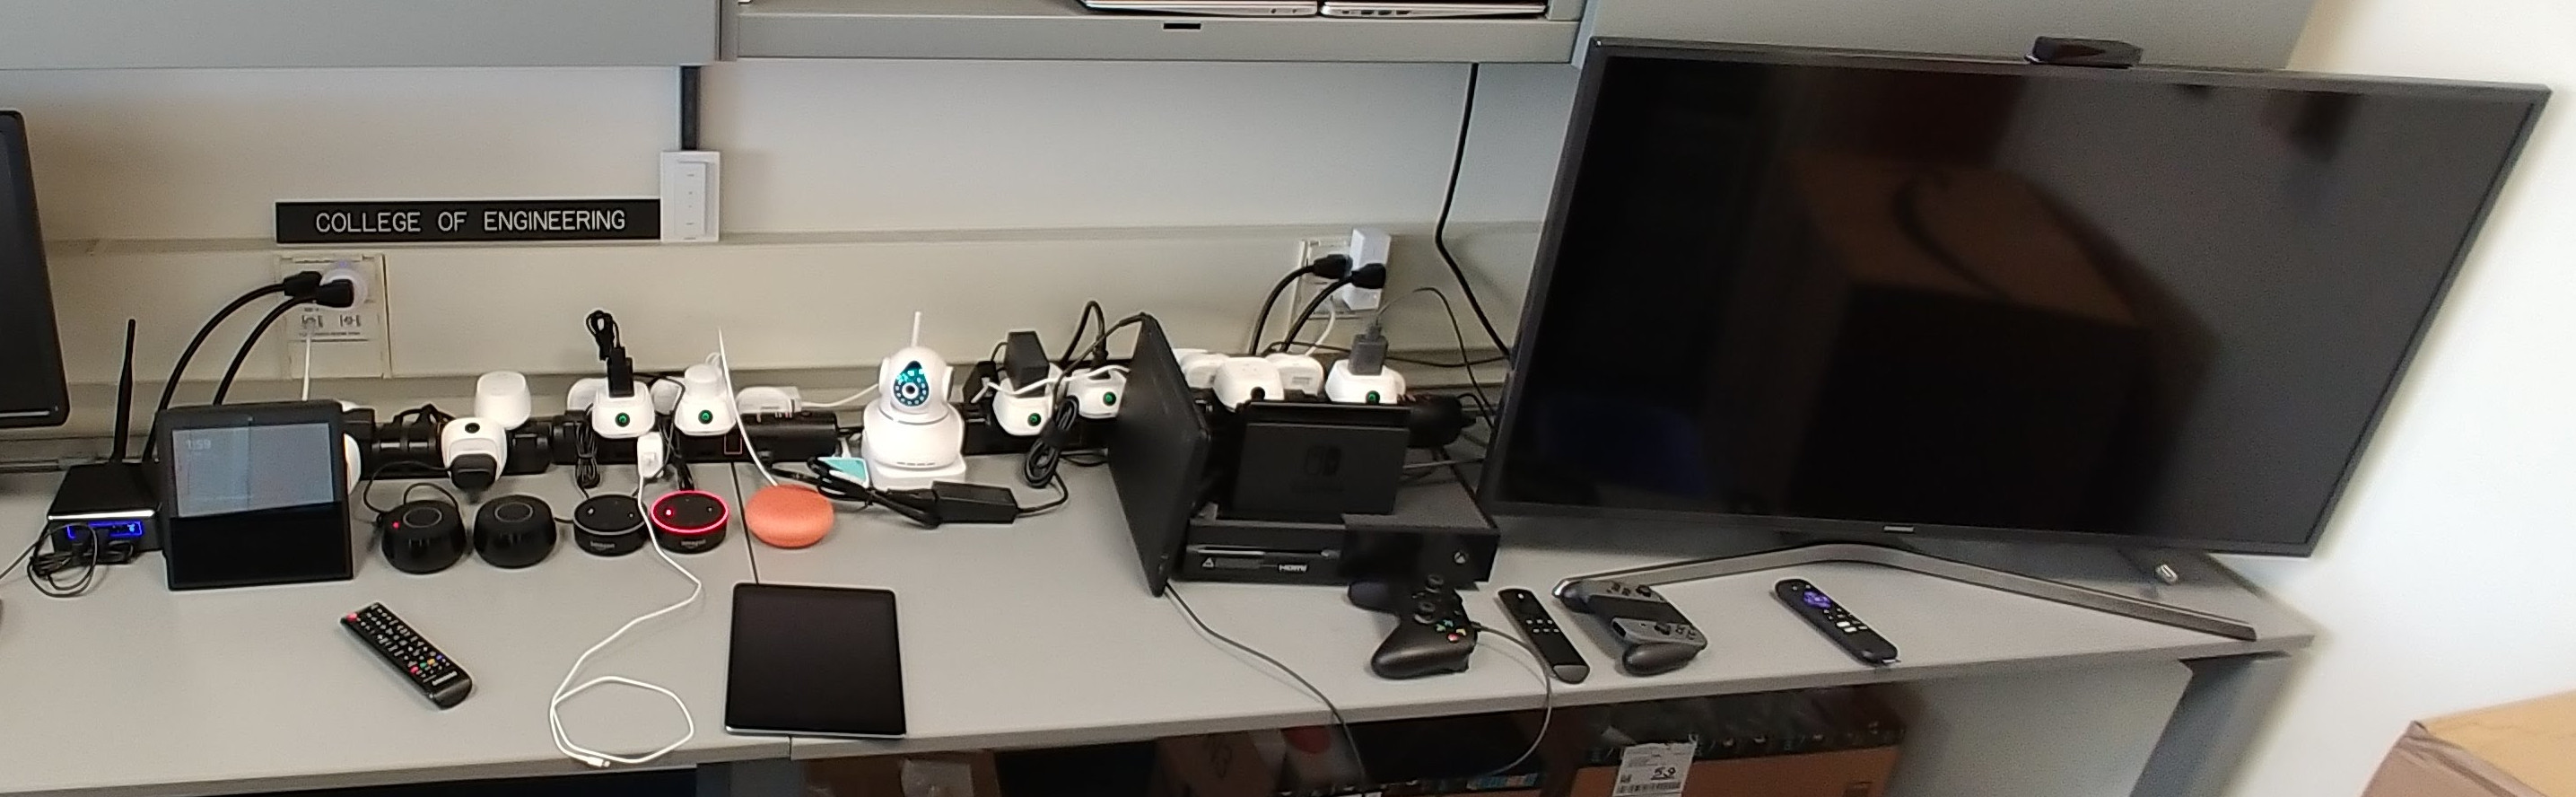
\includegraphics[width=1\textwidth]{devices}
    \caption{IoT Devices Under Examination}
    \label{fig:devices}
\end{figure}

\section{Physical Layout and Setup}
\label{Physical Layout and Setup}

This section covers the physical setup and layout of the hardware used when setting up the IoT test bed, the IoT devices we tested, and how each device is set up. Figures \ref{fig:wemo} and \ref{fig:devices} show the IoT testbed set up. Setup was performed with Ryan Frawley and explained in his paper \ref{frawleyPaper}, this paper provides an updated description.

\subsection{Wireless Access Point}
\label{Wireless Access Point}
The wireless access point is an Intel NUC \cite{nuc}. We loaded Ubuntu\cite{ubuntu} on it because its the most common Linux OS \cite{linux} and most flexible for developing scripts and programs to log network packets, query power information, and push those values to a database.

One challenging thing about the NUC is that its internal wireless chip is very slow. The throughput when using the wireless chip was measured to be 12 Mb/s down on Speedtest.net by Ookla \cite{speedtest} when connected to with a Chromebook \cite{chromebook} (25 Mb/s is the minimum possible for broadband). This rate limitation caused many of the Belkin Wemo smart switches \cite{wemo} to drop their connection intermittently, causing gaps in recorded power data. To solve this, we added a USB wireless antenna to the NUC. This antenna improved our internet speed to 30 Mb/s down when tested on Speedtest.net by Ookla with the same Chromebook, solving the issue where devices would lose network connectivity.

\subsection{Devices}
\label{Devices}
This section goes over the smart speakers, streaming devices, video game consoles, tablets, security cameras, or other devices as listed in figure \ref{tab:devices}. These devices were included based on their popularity, as the goal of the paper is to build a data set from common household IoT items.

\begin{table}[H]
    \centering
    \caption{IoT Devices Being Monitored}
    \begin{tabular}{@{}llll@{}}
    \toprule
    Category & Manufacturer & Device        & Quantity \\ \midrule
    Game Console & Nintendo     & Switch        & 1        \\
    Game Console & Microsoft    & Xbox One      & 1        \\
    Laptop & HP           & Chromebook    & 1        \\
    Media Player & Samsung      & Smart TV      & 1        \\
    Media Player & Google       & Chromecast    & 1        \\
    Media Player & Amazon       & Fire TV Stick    & 1        \\
    Media Player & Roku         & Express       & 1        \\
    Security Camera & Eray    & Hi3518 WiFi Camera     & 1        \\
    Smart Speaker & Amazon       & Echo Dot      & 2        \\
    Smart Speaker & Eufy/Anker   & Genie         & 2        \\
    Smart Speaker & Amazon       & Echo Show     & 1        \\
    Smart Speaker & Google       & Home Mini     & 1        \\
    Tablet & Amazon       & Fire 7 Tablet & 2        \\
    Tablet & Samsung      & Galaxy Tablet & 1        \\
    Tablet & Apple        & iPad          & 1        \\ \bottomrule
    \end{tabular}
    \label{tab:devices}
\end{table}

\subsubsection{Smart Speakers}
\label{Smart Speakers}

Smart speakers are IoT devices that combine speakers with built-in voice assistants, such as Amazon Alexa, Google Assistant, or Apple's Siri. These devices are mainly controlled by voice commands, preceded by a wake word such as ``hey Google''.

Currently, around 39 million people (16 percent of the US population) use smart speakers\cite{perez_2017}. It is one of the top-selling IoT devices and it can act a central voice control for other IoT devices. In 2022 it is projected that 70 million US households will have at least one smart speaker (55 percent of US households) and around 175 million smart speakers total\cite{perez_2018}. For these reasons, we included this group of devices in our research.

Within the smart speaker category, we included the Amazon Echo Dot, Google Home, and Eufy Genie. The Amazon Echo dot and the Google Home are the two leading smart speaker products. We added the Eufy Genie because it is a Amazon Alexa device that we can compare with the Echo Dot. We also included the Amazon Show, which is a voice assistant with a screen.

\subsubsection{Streaming Devices}

Streaming devices are IoT products that connect to a television or are built into a television (smart TVs) and streams videos or music from online services. In 2017 it was recorded that 70 million US households (58.7 percent of homes) had a television connected to streaming devices \cite{lynch_2017}.

The specific streaming devices we look at include the Roku Express, Amazon Fire TV, and the Google Chromecast. These devices represent three popular streaming platforms (Roku, Google Chromecast, Amazon Fire TV) that have a combined user base of over 110 million users who watch content at least once a month \cite{emarketer_2017}.

To view content from these streaming devices, we use a Samsung smart TV. This TV also as streaming capabilities which we log but do not analyze in this paper.

\subsubsection{Video Game Consoles}

Video game consoles are systems specifically built to play video games. We use two out of the three most popular gaming devices including the Nintendo Switch which sold 17.8 million units \cite{nintendo} and the Xbox One, which sold 30 million units \cite{souppouris_2016} as of January 2018.

\subsubsection{Tablets}

Tablets are devices that have phone operating systems running on them such as the Apple IPad, Samsung Galaxy tablet, and the Amazon Fire tablet. These devices were used for interacting with the other IoT devices, which require a smartphone or tablet for set up or control. Some of the IoT devices are limited to either Android, which runs on the Galaxy, or IOS, which runs on the IPad. Although there is no analysis on these devices in the paper, the netowork packets are logged. There is no way to track the power usage of these devices because they run on battery.

\subsubsection{Security Camera}

Security cameras are cameras meant to run constantly as surveillance, streaming the video footage so a user can view it from any connected device at any time. Two out of the five largest recorded cybersecurity attacks targeted security cameras \cite{guest_2018}. The specific camera we use is the Eray camera. It is a generic Alibaba device with a weak username:password of admin:1234. A weak username and password makes it very susceptible to cyber attacks. There have also been reports that smart cameras have been found to send unencrypted data \cite{feamster_2016}. We selected this device because it has weak login credentials and is susceptible to Mirai. We wanted to see if it would get hacked by Mirai or some other attack, but we found no indication of such.

\subsubsection{Other Devices}

We also connected several other devices that are harder to categorize, analyze, or both.

We have a smart hub connected to a smart lock, an indoor room temperature sensor, and smart LED light bulbs. These devices are difficult to analyze because they communicate with the smart hub through Zigbee or Bluetooth at which point the smart hub aggregates the data and communicates with the network. In order to look at the network traffic caused by smart lights individually, we prevented all devices besides the smart LED bulbs from communicating with the smart hub. This isolation minimized other packet noise to the smart hub so that we can monitor the smart hub traffic as a replacement for the smart LED bulbs. However, even then, the smart hub might have extra overhead for other tasks, making isolated analysis difficult.

We also have a Chromebook which we used to control the Chromecast. However, because this is more a laptop than an IoT device, we decided to leave this out of our research

\subsection{Smart Power Plugs}

Smart power plugs are WiFi capable, pass through outlets that another device plugs into. The outlets collect and transmit power usage over the network. They are critical to the power consumption logging in this research.

We used the Belkin Wemo Insight. We chose this smart plug because there are many open source Python libraries for pulling power information from them, and they are relatively affordable.

When setting these smart plugs up, we named each smart plug based on the device connected to it so that when we pull power information with our scripts, we can easily reference data to a smart plug. This informal naming led to issues when the wrong device is connected to the wrong smart plug, as discussed in section \ref{realtimeIoTGrapher.py}

\subsection{Wiring and Configuration}

We also tried to set static IPs for each device, but we decided that the average user would not set up a static IP for their device and left dynamic IPs.

The next step was to setup each device and corresponding smart plug through their corresponding setup application, filling in the device's, user name, email, network configuration, and etc. We used the device's name as its user name, e.g. the Echo Dot was given the username ``Echo Dot''.

When plugging in all of the devices for the first time for power, we worked to plug each device into the corresponding Wemo smart plug and connected to our WAP during device set up so that we could instantly log power and network traffic information. It was essential to log power as soon as possible to capture a first-boot power profile for each device. Some devices had already been used, so they do not contain startup information(Xbox and the Echo Dot 1).

Set up and configuration took up a significant portion of the research time. We worked to set up each device with a separate email account. To do this, we made around 20 AOL accounts. We wanted email addresses that were not under control of the manufacturer of any of the devices. For example, we did not want to use any Gmail accounts because we did not want the Google Home or Google Chromecast to perform domain-specific optimizations. When setting up AOL accounts, we also faced a limitation of the number of email accounts tied to a single phone number. We had to use different phone numbers to circumvent this.

We set up each device in waves, taking around a week to set everything up. Incremental device setup with no plan resulted in a messy work environment, which made it difficult to match a device to it is corresponding smart plug. After a month of data logging in a disorganized scheme where it was difficult to keep track of each device, we unplugged everything, renamed the Wemos, organized the wiring, and organized the location of each smart device resulting in the set up in figures \ref{fig:wemo} and \ref{fig:devices}. With limited power strips, the organization helped maximize power ports. We also made sure to face the button for each power plug towards our view so that we could quickly notice whether the power plugs were on or off. Organization streamlined the logging process in the long run; debugging network and connection issues was much simpler with an ordered set up. We could quickly identify redundant devices (there are two Echo Dots and Eufy Genies), run procedures on groups of devices, and determine the corresponding smart plug for each device.

\section{Software}
\label{software}
This section covers the software components used to control the IoT test bed. It discusses the scripts for logging power and network traffic, the database information, and the python script for visually viewing the database.

\subsection{Wireless AP Code}
In order to turn the NUC into a wireless access point, we used a create\_ap script \cite{oblique_2017}. This app takes in the WiFi name, WiFi password, and the wireless interface. This script turned the NUC into a wireless access point (WAP). We later found that, with newer versions of Ubuntu, there is a built-in feature for creating a hotspot through a wireless interface on the device \cite{m_2016}. We later used this feature to simplify the amount of programs running and instead have a the OS handle the hotspot. Partially through our research, as we set up more IoT devices and demand for bandwidth through the WAP increased, we had to switch to an external antenna and rerun the script in order to set the USB antenna as the WAP wireless interface. During this time, there is a void in network and power entries in the database.

\subsection{sniff.py}
\label{sniff.py}

Sniff.py runs a thread for power logging and a thread for network logging. As each logger runs, it writes the network packets and power information to a MySql database hosted on AWS through the python mysqlclient \cite{mysqlclient} library. If the database connection is lost, the script automatically reconnects.

\subsubsection{Network Logging}

It begins by opening a socket on the wireless interfaces connected. All IP packets are sniffed through this socket connection as shown in listing \ref{lst:sock}.

\begin{minipage}{\textwidth}
\begin{lstlisting}[label={lst:sock},caption={Open and Read from a Socket},captionpos=b]
self.socket = socket.socket(socket.AF_PACKET, socket.SOCK_RAW, socket.htons(ETH_P_ALL))
self.socket.setsockopt(socket.SOL_SOCKET, socket.SO_RCVBUF, 2**30)
self.socket.bind((self.interface_name, ETH_P_ALL))
while True:
    packet, address = self.socket.recvfrom(MTU)
\end{lstlisting}
\end{minipage}

Once we have sniffed a packet, we can obtain the metadata from the hex dump. We preserve this hex dump because in case we would want to extract more information from it later on. From each hex dump, we extract and store the source IP, source host, destination IP, destination host, time, size, type, protocol, source port, destination port, source host, destination host, and hex dump. We will explain what each field in section \ref{Database}.

\subsubsection{Power Logging}

The second addition to our IoT device analysis is the power information. To obtain this information, we rely heavily on the Belkin Wemo Insights. Each Wemo connects to an outlet and each IoT device plugs into the Wemos.

We used the PyWemo python script \cite{pywemo} to read power usage from the Wemos once per second. This is the highest frequency we could poll for power. The Wemo is capable of reading both power and energy in mW and kW hours.

Once the script queries the Wemo for its power information, we relate the Wemo to the device connected to it by extracting the name of the Wemo. This information is used when pushing power data to our database.

One issue with PyWemo and the Belkin Wemos was that they would sometimes disconnect and the script would miss out on power data. To solve this issue, the script rescans for Wemos until it finds all 16 Wemos in our testbed. The rescan code for this is shown below in listing \ref{lst:wemoRescanCode}

\begin{minipage}{\textwidth}
\begin{lstlisting}[label={lst:wemoRescanCode},caption={Rescan if all wemos not found.}]
    def scan_until_all_found():
        print("Discovering Wemos")
        switches = pywemo.discover_devices()
        print("Discovered {} switches".format(len(switches)))
        print(switches)
        try_num = 1

        while len(switches) < 16:
            print("Did not discover enough switches, trying again{}...".format(try_num))
            switches = pywemo.discover_devices()
            try_num += 1
            print("Discovered {} switches".format(len(switches)))

        return switches
\end{lstlisting}
\end{minipage}

\subsection{Database}
\label{Database}

To store all the result of the sniffed packets and power data, we push the data to a MySQL database hosted on an Amazon AWS server. As of writing, the database holds 172,445,929 entries that take up 184.94 GB of space. To interface with our database, we used a combination of the RealTimeIoTGrapher from section \ref{realtimeIoTGrapher.py}, Navicat \cite{navicat}, and mysql's commandline tool \cite{mysqlCommandline}.

\subsubsection{Network Table}

The largest part of our database is the IP network table. This table contains all the network packets that have gone through the NUC WAP. It is currently 179.1 GB and contains 116,830,077 entries. It is so large because it consists of all network traffic generated over a 12 month period. In those 12 months, we did many high bandwidth tasks such as playing music or video. These entries contain the raw hex dump of the whole packet, which contains all the metadata plus data load, further contributing to the massive size of this table. The data table's rows represent a single packet with the columns shown in the table below \ref{tab:netcol}.

\begin{table}[H]
    \centering
    \caption{Columns in Network Traffic Table}
    \begin{tabular}{@{}lll@{}}
    \toprule
    Column Number & Column Name & Data Type \\ \midrule
    1             & time        & datetime  \\
    2             & source      & varchar   \\
    3             & src\_host   & varchar   \\
    4             & destination & varchar   \\
    5             & dst\_host   & varchar   \\
    6             & protocol    & varchar   \\
    7             & type (in/out)       & varchar   \\
    8             & src\_port   & varchar   \\
    9             & dst\_port   & varchar   \\
    10            & size        & int       \\
    11            & hexdump     & longtext  \\ \bottomrule
    \end{tabular}
    \label{tab:netcol}
    \end{table}

Common SQL commands we used for our analysis include those shown in listings \ref{fig:navicatPowerQuery} and \ref{fig:navicatNetworkQuery}. The most useful commands generally required examining total throughput or device throughput using ROLLUP, shown in figure \ref{fig:navicatRollup}.

\begin{figure}[H]
    \centering
    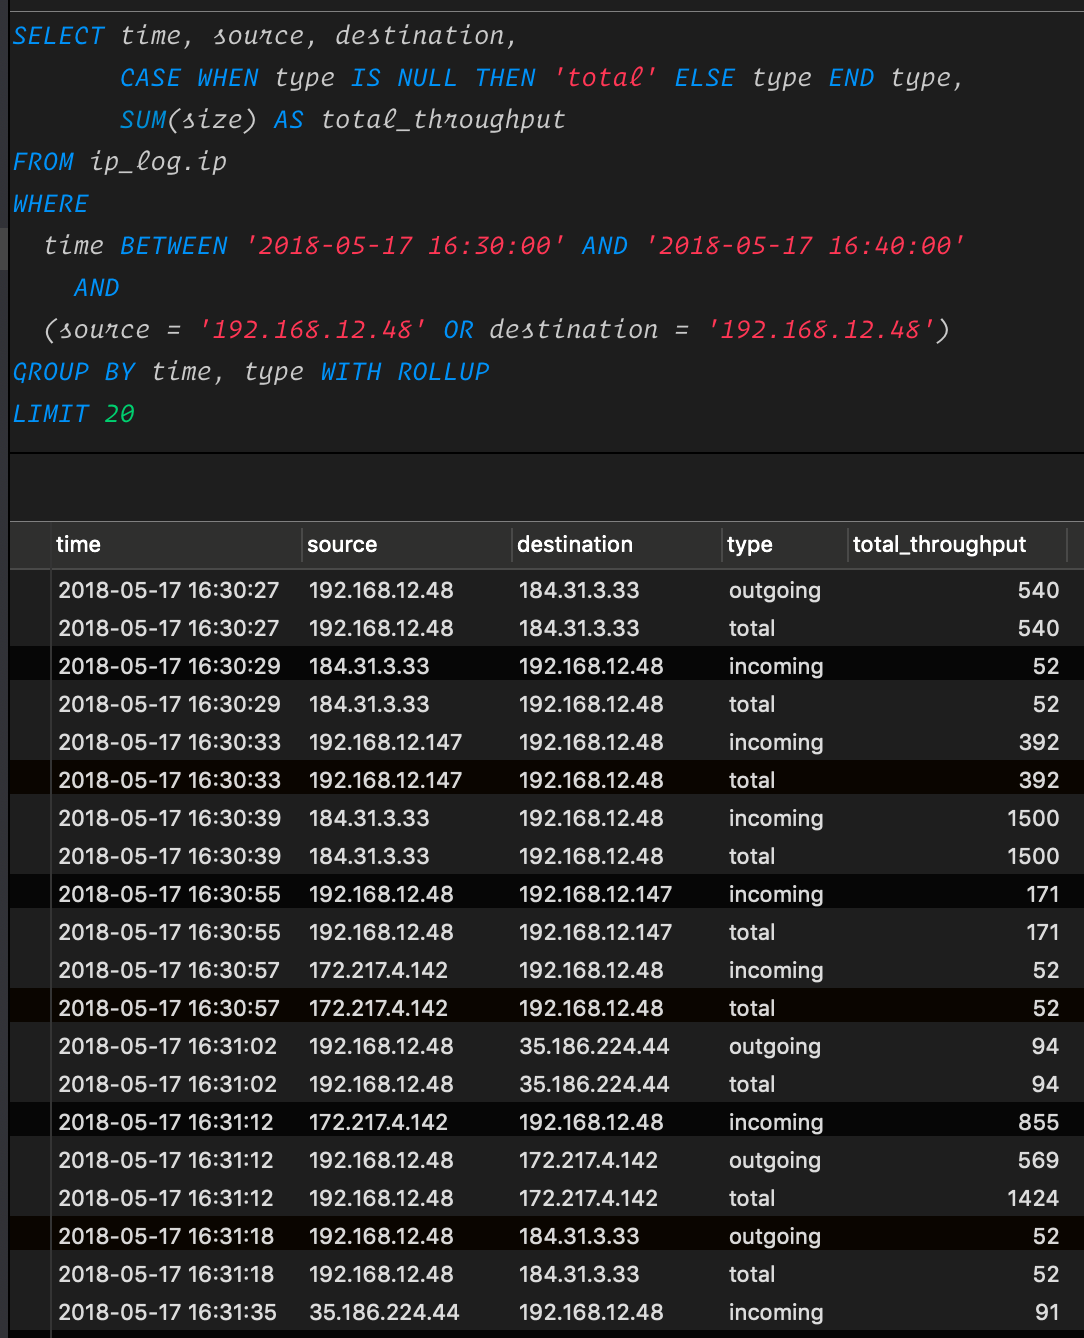
\includegraphics[width=1\textwidth]{figures/navicatRollup.png}
    \caption{Navicat ip query with rollup.}
    \label{fig:navicatRollup}
\end{figure}

The hex dump column drastically increases the size of each entry in the network table. However, as a raw network packet, it is very flexible and can be manipulated for many more use cases than the targeted columns we have. This flexibility is usefule for future research, that may require data we did not explicitly pull out for this project

In the database, each device can be tracked down by looking for the IP address of that device in the source or destination columns. However, note that during set up, we did not set up static IPs for these devices. Because of this, a single device can be under multiple IPs within the table. We ignored this issue until a query for a particular IP stopped working. At which point we would invoke a command on the device whose IP changed to flood the database with packets from that device, query the database in the time frame of the command, and obtain the new IP. We logged all devices and their current IP in a Google Sheets \cite{googleSheets} file covered in subsection\ref{Device Inventory}.

\subsubsection{Power Table}

The power table holds the most important data for this portion of the research, and we refer to it for the majority of the paper's findings. The size of this table is much smaller than the network table. It contains 5.84 GB of data and 61,240,189 entries in the database. The large difference in size between the IP table and power table is because each device only produces one entry power entry every second. The columns of the power table are shown below in figure\ref{tab:powcol}.

\begin{table}[H]
    \centering
    \caption{Columns in Power Table}
    \begin{tabular}{@{}lll@{}}
    \toprule
    Column Number & Column Name     & Data Type \\ \midrule
    1             & name            & varchar   \\
    2             & power\_mw       & int       \\
    3             & time            & datetime  \\
    4             & today\_kwh      & varchar   \\
    5             & on\_for         & varchar   \\
    6             & today\_on\_time & varchar
    \end{tabular}
    \label{tab:powcol}
    \end{table}

When working with this database, we generally query for a range of power packets in a given time range. We do this for either all devices, a subset of devices, or a single device. Some of the commands and results are shown below in figures \ref{fig:navicatPowerQuery} and \ref{fig:navicatNetworkQuery}.

\begin{figure}[H]
    \centering
    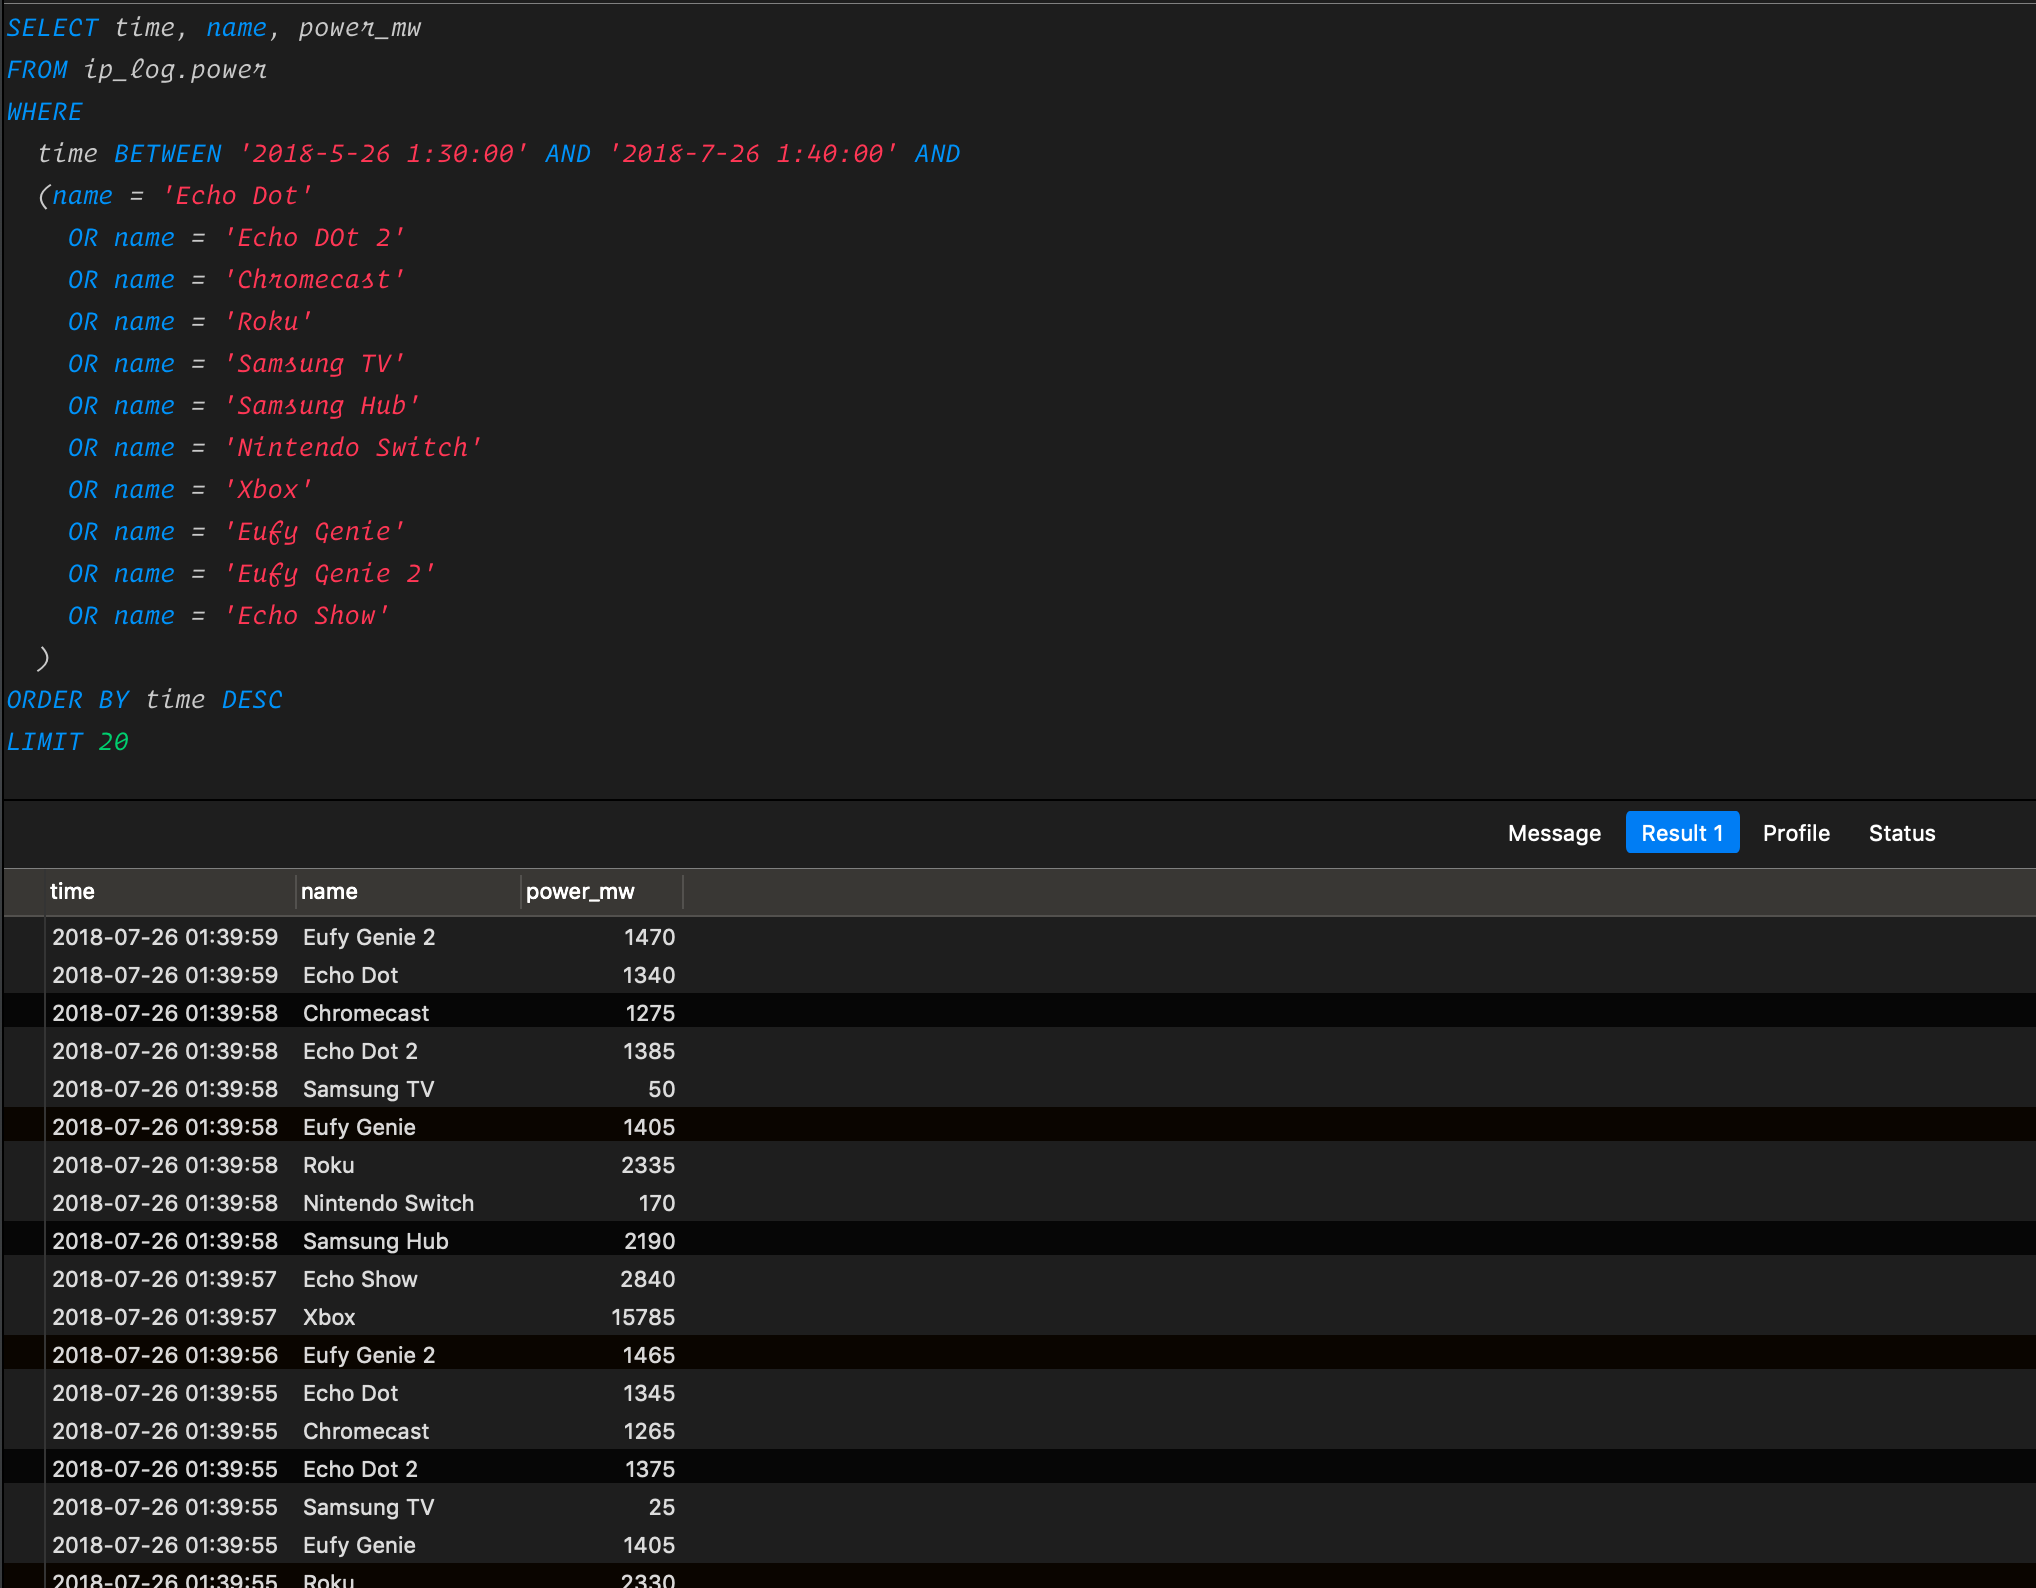
\includegraphics[width=1\textwidth]{figures/navicatPowerQuery.png}
    \caption{Power query from database with Navicat.}
    \label{fig:navicatPowerQuery}
\end{figure}

\begin{figure}[H]
    \centering
    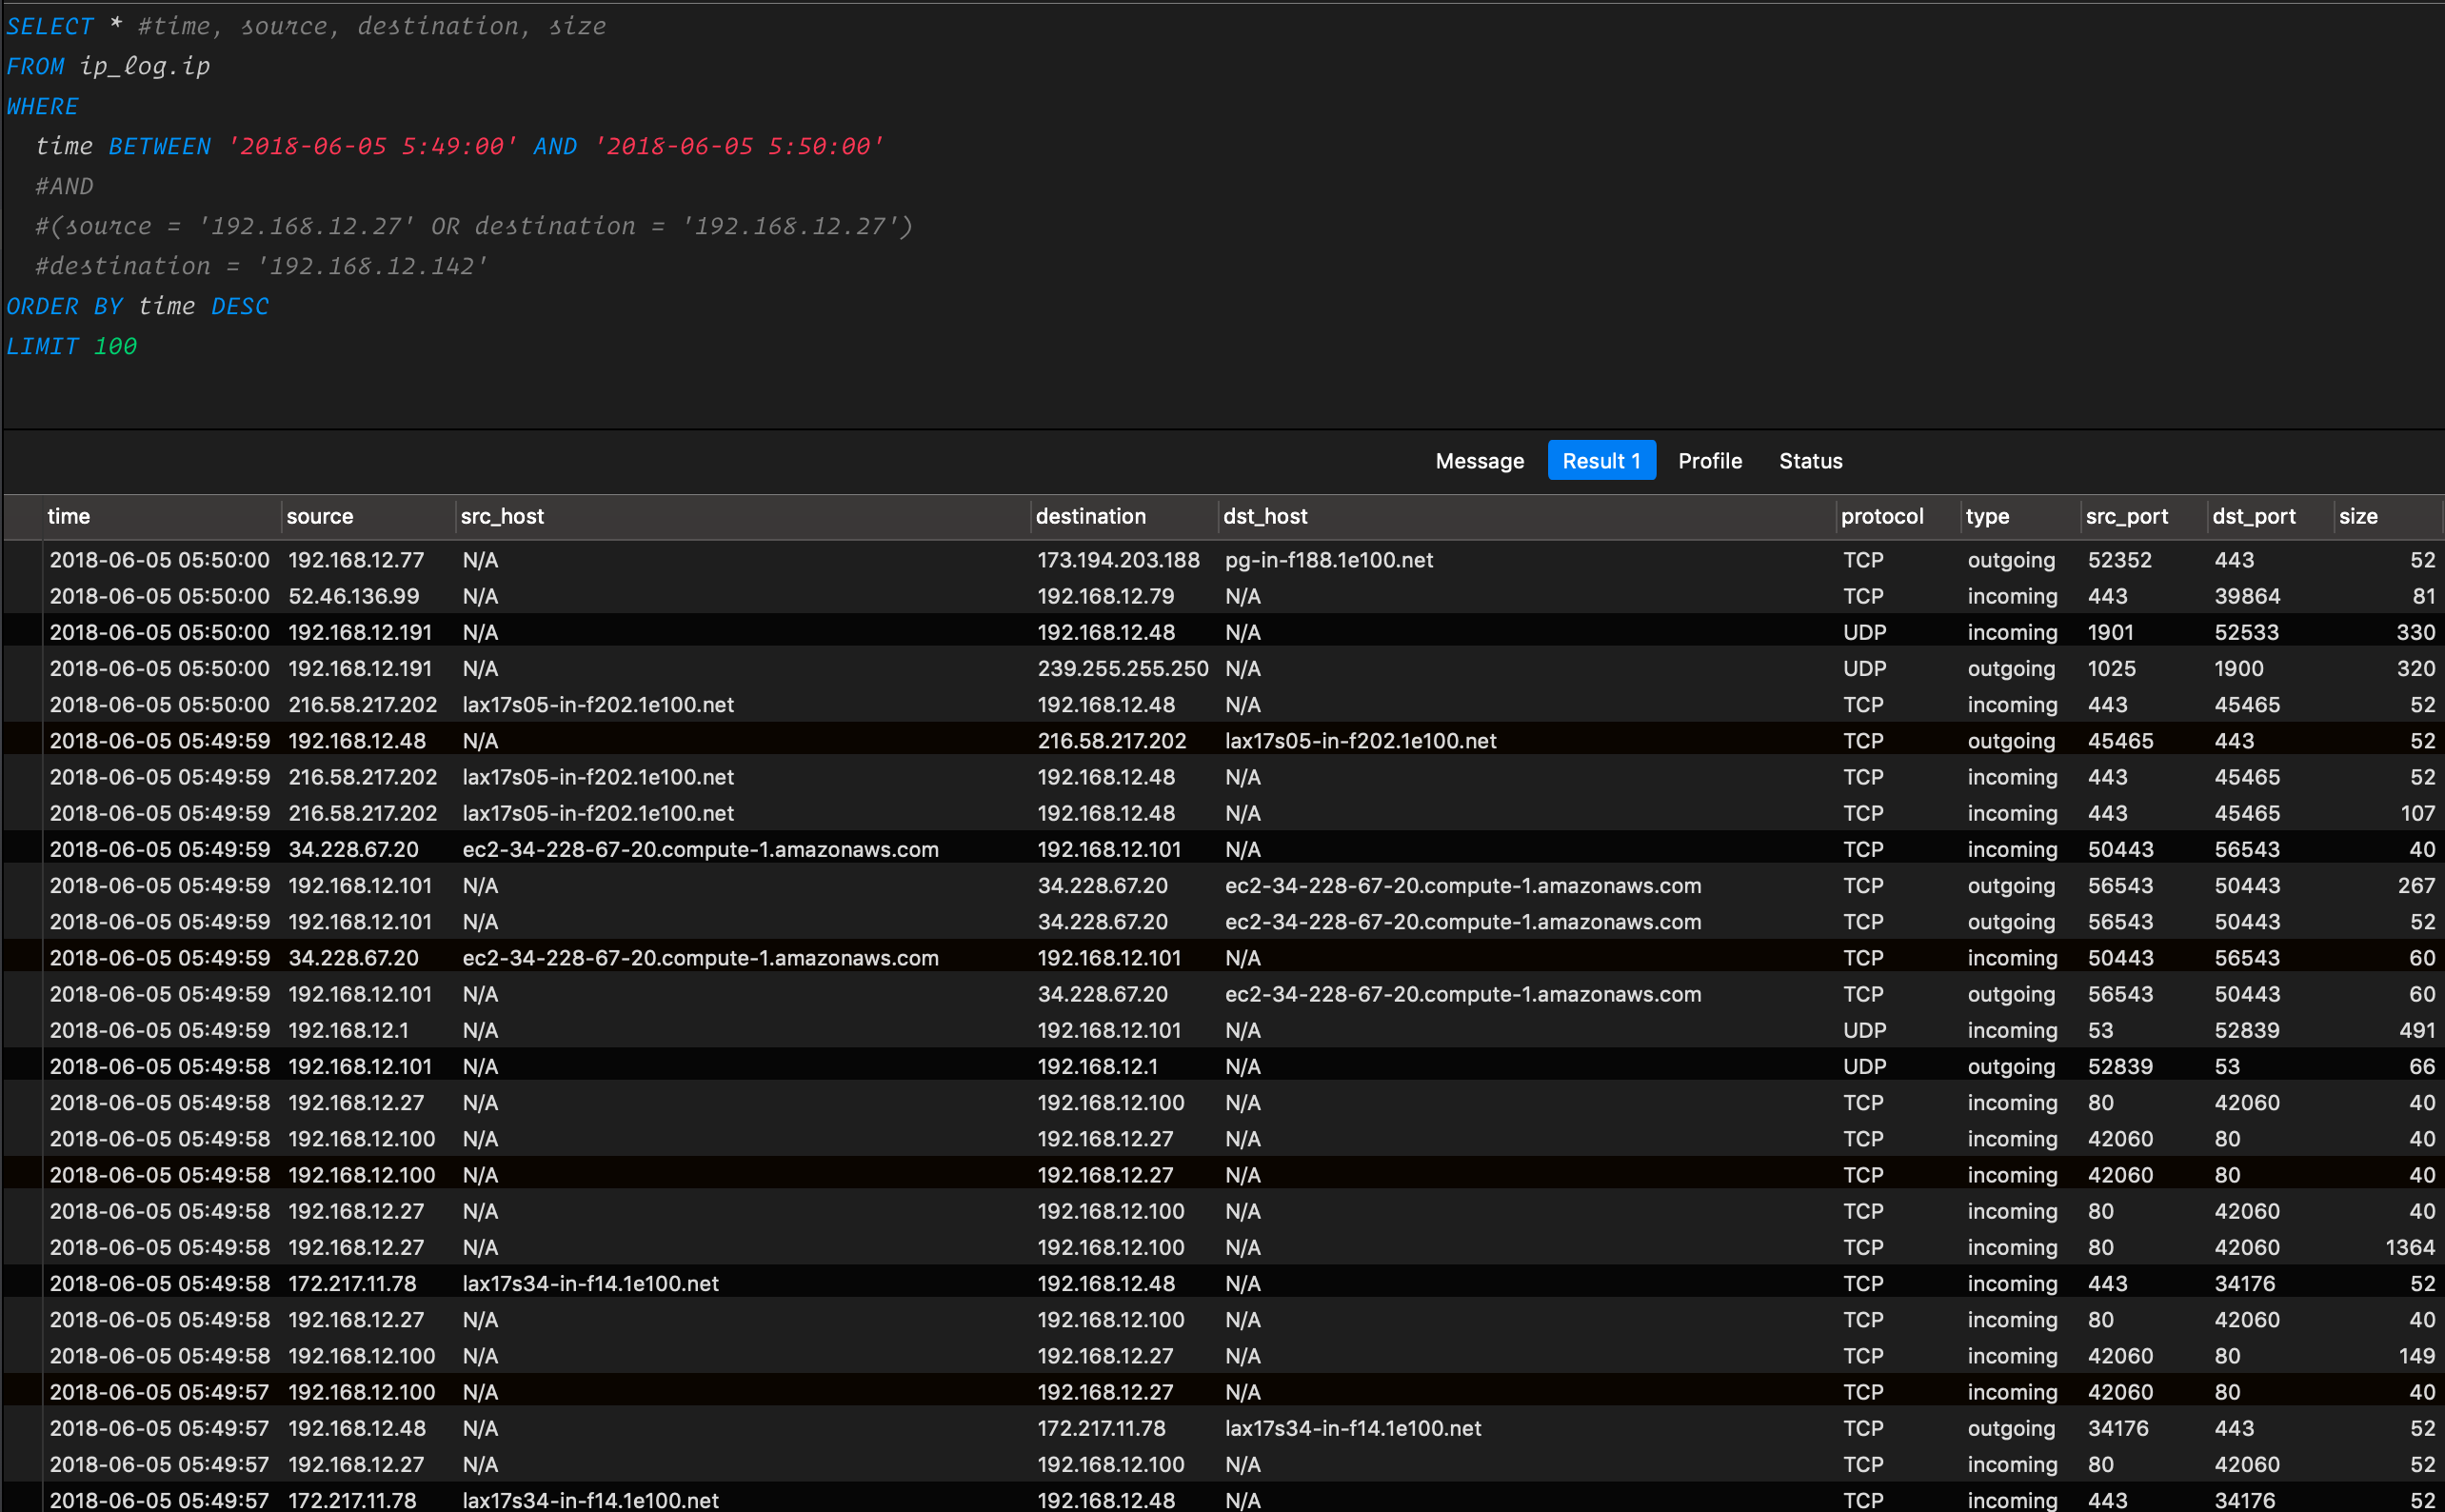
\includegraphics[width=1\textwidth]{figures/navicatNetworkQuery.png}
    \caption{Network query from database with Navicat.}
    \label{fig:navicatNetworkQuery}
\end{figure}
Within the power table, the name field is extracted from the name of the Wemo, which we manually name through the app. This can cause issues if the wrong device is connected to a Wemo. For example, the Echo Dot could have accidentally been connected to the Wemo named Google Home. There is no way to check for this besides manual examination, which we did after a few weeks, resetting all devices and causing a temporary void in power data. When we reset all devices, we also renamed some of the Wemos. For example, we changed ``echoDot'' to ``Echo Dot''. This way, all devices would follow the naming convention of separating words with spaces and capitalizing each word. Another possible naming convention could have been to name the Wemo by the IPs of the devices they connect to, but they are not static.

The sampling frequency for the power table is also low and missing some points. The script to query power data is not consistent and is unable to get power data at every second. To handle missing points, I interpolate them as shown in subsection \ref{realtimeIoTGrapher.py}. The interpolation process may introduce imprecise data as it fills a missing datapoint by extrapolating a linear path from the closest points before and after it.

\subsection{Device Inventory}
\label{Device Inventory}
To keep track of all devices and important details about them, we log a device's service, distributor, related email, IP address, dependencies, previous usage, and password into a Google Sheets file. An example of entries into the Device Inventory are shown below in table \ref{tab:deviceInventory}. The service field denotes the service a device provides, for example, the Google Home is a smart speaker. The device field denotes the specific manufacturer and device name. The Email and password fields denotes the email and password used when setting up the device. Some devices such as the Nintendo Switch were setup without an account. The IP address field denotes the ip address of the device within our local network. The dependencies field denotes anything the device is connected to or uses. For example, the Roku express is connected to a Wemo for power logging and comes with a controller for use. The used flag denotes whether the device was previously used or not, at which point, we could not log first time startup data for that device.

\begin{table}[H]
    \centering
    \caption{Device inventory excerpt. Password column not shown.}
    \resizebox{\linewidth}{!}{%
    \begin{tabular}{@{}lllllll@{}}
        \toprule
        Service      & Device            & Email                       & IP Address     & Dependencies     & Used \\ \midrule
        Speaker      & Amazon Echo Dot 1 & amazonEchoDotSS0@aol.com    & 192.168.12.79  & wemo             & yes  \\
        Speaker      & Google Home       & googleHomeMiniSS0@aol.com   & 192.168.12.48  & wemo             & no   \\
        Streaming    & Google Chromecast & googleChromecastSD0@aol.com & 192.168.12.78  & wemo             & no   \\
        Streaming    & Roku Express      & rokuExpressSD0@aol.com      & 192.168.12.68  & wemo, controller & no   \\
        Game Console & Nintendo Switch   & n/a                         & 192.168.12.160 & wemo, controller & no   \\ \bottomrule
        \end{tabular}}
    \label{tab:deviceInventory}
\end{table}


\subsection{Usage Flow}

One of the goals of this work is to create a data set that represents the baseline of normal network traffic and power usage. To do this, we used each IoT device at least twice a week for the year length of this research. To build a proper dataset that other people could use for research, we set up a list of things that we should do for each device interfacing with it. We logged the activities into Google Sheets so that these events could be correlated to entries in the database, giving context when looking back on this data. For example, if someone were to look at the database and notice that the power and network traffic was high for 3 minutes, they could look at our logs and see that the device was streaming music for those 3 minutes and assume that it was normal usage.

When logging events into Google Sheets, we include the start, end time, name of the device(s), action performed, and any individual notes. When naming the devices, we used the same naming as we did for the Wemos in order to maintain consistency from the log to the database. An example of entries into the table is shown in Table \ref{tab:events}.

\begin{table}[H]
    \centering
    \caption{Event Log Excerpt}
    \begin{tabular}{@{}lllll@{}}
        \toprule
        Date & Start Time & End Time & Device & Event \\ \midrule
        5/25/2018 & 12:44:42 & 12:47:04 & Home Mini & Ask for news \\
        5/25/2018 & 12:55:07 & 12:56:37 & Echo Dot & Ask for news \\
        5/25/2018 & 12:55:57 & 12:56:17 & Echo Show & Ask for weather \\
        5/25/2018 & 12:56:44 & 13:03:07 & Home Mini & Play music \\ \bottomrule
        \end{tabular}
    \label{tab:events}
\end{table}

The following subsections explains the script created to automate the event logging portion of the research. Then it explains the specific procedure we ran each group of IoT devices through whenever we interfaced with them.

\subsubsection{Google Sheets Script}

Logging information into the spreadsheet is a tedious task, especially when trying to analyze each device while running tasks on them. The code for the script is shown below in Listing~\ref{lst:sheetScript}.

\begin{minipage}{\textwidth}
\begin{lstlisting}[basicstyle=\linespread{0.95}\ttfamily, language=C,label={lst:sheetScript},caption={Open and Read from a Socket}]
function onEdit() {
  var s = SpreadsheetApp.getActiveSpreadsheet().getSheetByName("Event Log");
  var r = s.getActiveCell();
  var c = r.getColumn();

  if( c == 4 || c == 5) { // checks the column
    var dateCell = r.offset(0, -3);

    if( dateCell.getValue() === '' ) {// is empty?
      var startTimeCell = r.offset(0, -2);

      // fill in the start time and date
      var date = new Date();
      dateCell.setValue(date);
      startTimeCell.setValue(date.toLocaleTimeString());
    }
  }

  if( c == 6 ) { // checks that the description is being entered
    // if so fill in the end time
    var endTimeCell = r.offset(0, -3);

    if ( endTimeCell.getValue() === '' ) {
      endTimeCell.setValue(new Date().toLocaleTimeString());
    }
  }
}
\end{lstlisting}
\end{minipage}

\subsubsection{Smart Speakers}

Whenever interfacing with these devices, we always queried for the weather and the news. The specific phrases we used ``$<$wakeword$>$ what's the weather'' and ``$<$wakeword$>$ what's the news'', we  set a reminder for a random task in a random timeframe, and we muted the devices for a few minutes to see if they were still listening if we said the wake word.

\subsubsection{Video Game Consoles}

When interfacing with these devices, we played a game on the device for at least 15 minutes. Every week, we also browsed for games on the game store and downloaded free demos.

Afterward, we would turn off the Xbox and put the Nintendo Switch into sleep mode. The Nintendo Switch could not be put to sleep when docked, only when disconnected from the dock, so it was set to sleep rather than power off.

\subsubsection{Streaming Devices}

Within the Media Players section, we include the Roku Express, Chromecast, Amazon Firestick, and Samsung Smart TV. When interfacing with these devices, we watched youtube for at least either one video or 3 minutes.

For the Chromecast, we cycled through different devices to cast videos from, including the Ipad and the Chromebook. We wanted to get varied data in case the Chromecast prioritized streaming from different devices.

\subsubsection{Tablets}
In this experimental setup, we used the tablets less for investigative purposes, but more to set up and interface with other devices.

However, we still tracked the data and had a small set list of things to do on these devices. We used each tablet to browse the web, watch YouTube, and use various apps.

\subsubsection{Security Camera}

The only security camera we worked with was the Eray Security Camera.

Whenever interfacing with this device, we used the device under the app NVAS2 in the IPad for at least 2 minutes. Usage included streaming video from the camera to Ipad and viewing it. We also controlled the camera through the app with pan and tilt commands. When done experimenting with the security camera, we disconnected the tablet from the camera by using the ``end stream'' button in the NVAS2 app.

\subsection{realtimeIoTGrapher.py}
\label{realtimeIoTGrapher.py}

This section covers a visual tool I created to look for trends. We initially graphed the data into Google Sheets and graphed it. The tables and formulas are shown in figure \ref{fig:excelLogging}. This process was tedious and time-consuming. We had to copy the data over after making a SQL query, extract unique time values, and then get the total network and power usage at each time interval.

To address these problems, I created a python script that automatically forms graphs, including the one shown in figure \ref{fig:interpolated} when given the time range and the devices. This automation sped up the analysis process and provided extra features covered in section \ref{Features}.

This Python script leverages the Plotly library, which, given data, will graph it onto a local web page for viewing. Plotly comes with many useful tools for further analysis and can be extended to run on a public web page for public viewing.

I plan to distribute this out with our database so that researchers can view the power and network information of any device at a glance.

\begin{figure}[H]
    \centering
    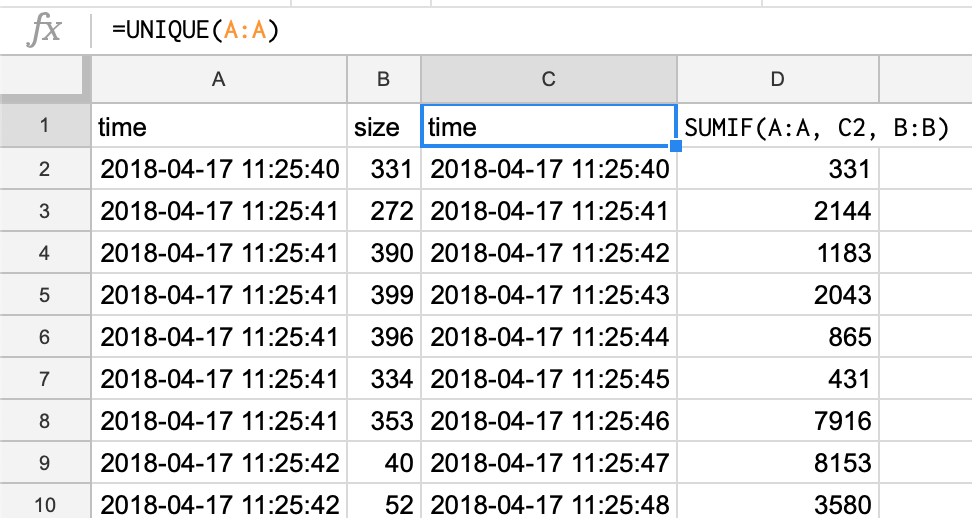
\includegraphics[width=1\textwidth]{excelLogging}
    \caption{Manual Analysis of IoT devices in Google Sheets: Raw data shown in columns A and B are then formatted into columns C and D for Graphing}
    \label{fig:excelLogging}
\end{figure}

\begin{figure}[H]
    \centering
    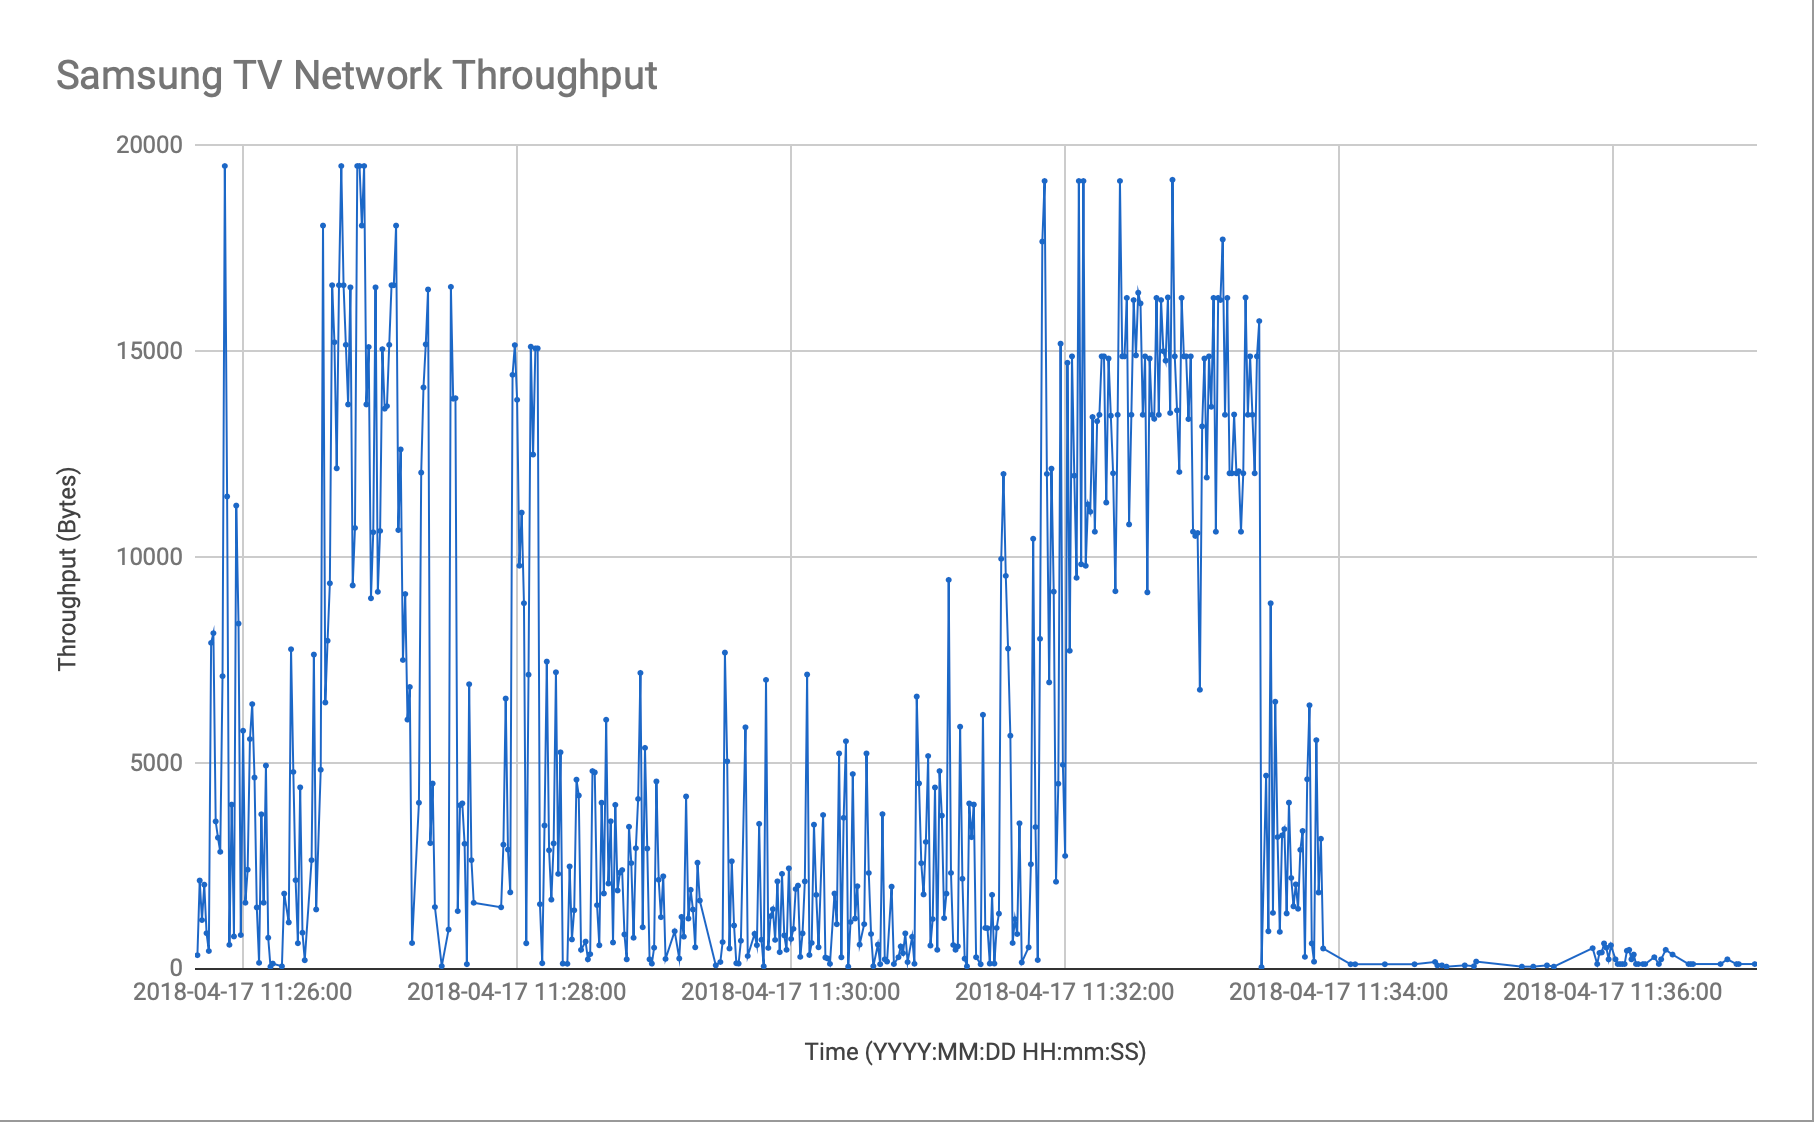
\includegraphics[width=1\textwidth]{figures/tvThroughput.png}
    \caption{Resulting graph of dataset shown in Figure \ref{fig:excelLogging}}
    \label{fig:tvThroughput}
\end{figure}

\subsubsection{Features}
\label{Features}

This section, discusses the features that RealTimeIoTGrapher (grapher) provides.

At its core, this program automates the creation of the graph shown in figure \ref{fig:tvThroughput}. The user can specify a time range that the graph should cover and what devices to graph. By default the graph shows power, input traffic, output traffic, and total network traffic over the time range specified.

The grapher also annotates the data by including a line denoting the average for each of the traces over the time range currently displayed. It also annotates the maximum and minimum values in the time range for each trace. The grapher can also display information in real time for an user settable interval amount of time, updating every second.

The Plotly libraries also provide useful tools when displaying these IoT graphs. It is possible to zoom in and out the displayed graph, select specific traces for viewing, save the graph, and hover over data points to display the specific value. Finally, once a graph is saved Plotly allows further editing of the graph so that it is formatted the way the user wants.

\begin{minipage}{\textwidth}
    \begin{lstlisting}[language=SQL, label={lst:rollup},caption={Efficient SQL query to obtain total Network throughput at each second.}]
    def throughput_query_in_range(db_connection, device, start_time, end_time):
    sql_query = """
        SELECT
            time,
            CASE WHEN type IS NULL THEN 'total' ELSE type END type,
            SUM(size) AS total_throughput
        FROM ip_log.ip
        WHERE
            time BETWEEN '%s' AND '%s' AND
            (source = '%s' OR destination = '%s')
        GROUP BY time, type WITH ROLLUP;
    """ % (start_time, end_time, ip[device], ip[device])

    dataframe = pd.read_sql_query(sql_query, db_connection)

    return dataframe
    \end{lstlisting}
\end{minipage}

To reduce local computation, the grapher offloads work to the server through a SQL query. When querying for network data, it performs a SQL ROLLUP in order to sum the incoming and outgoing network throughput to obtain the total throughput. ROLLUP is required because it provides nested queries and causes the query to sum up the data by time for each type of packet. This query is formatted as shown in listing \ref{lst:rollup}.

\begin{figure}[H]
    \centering
    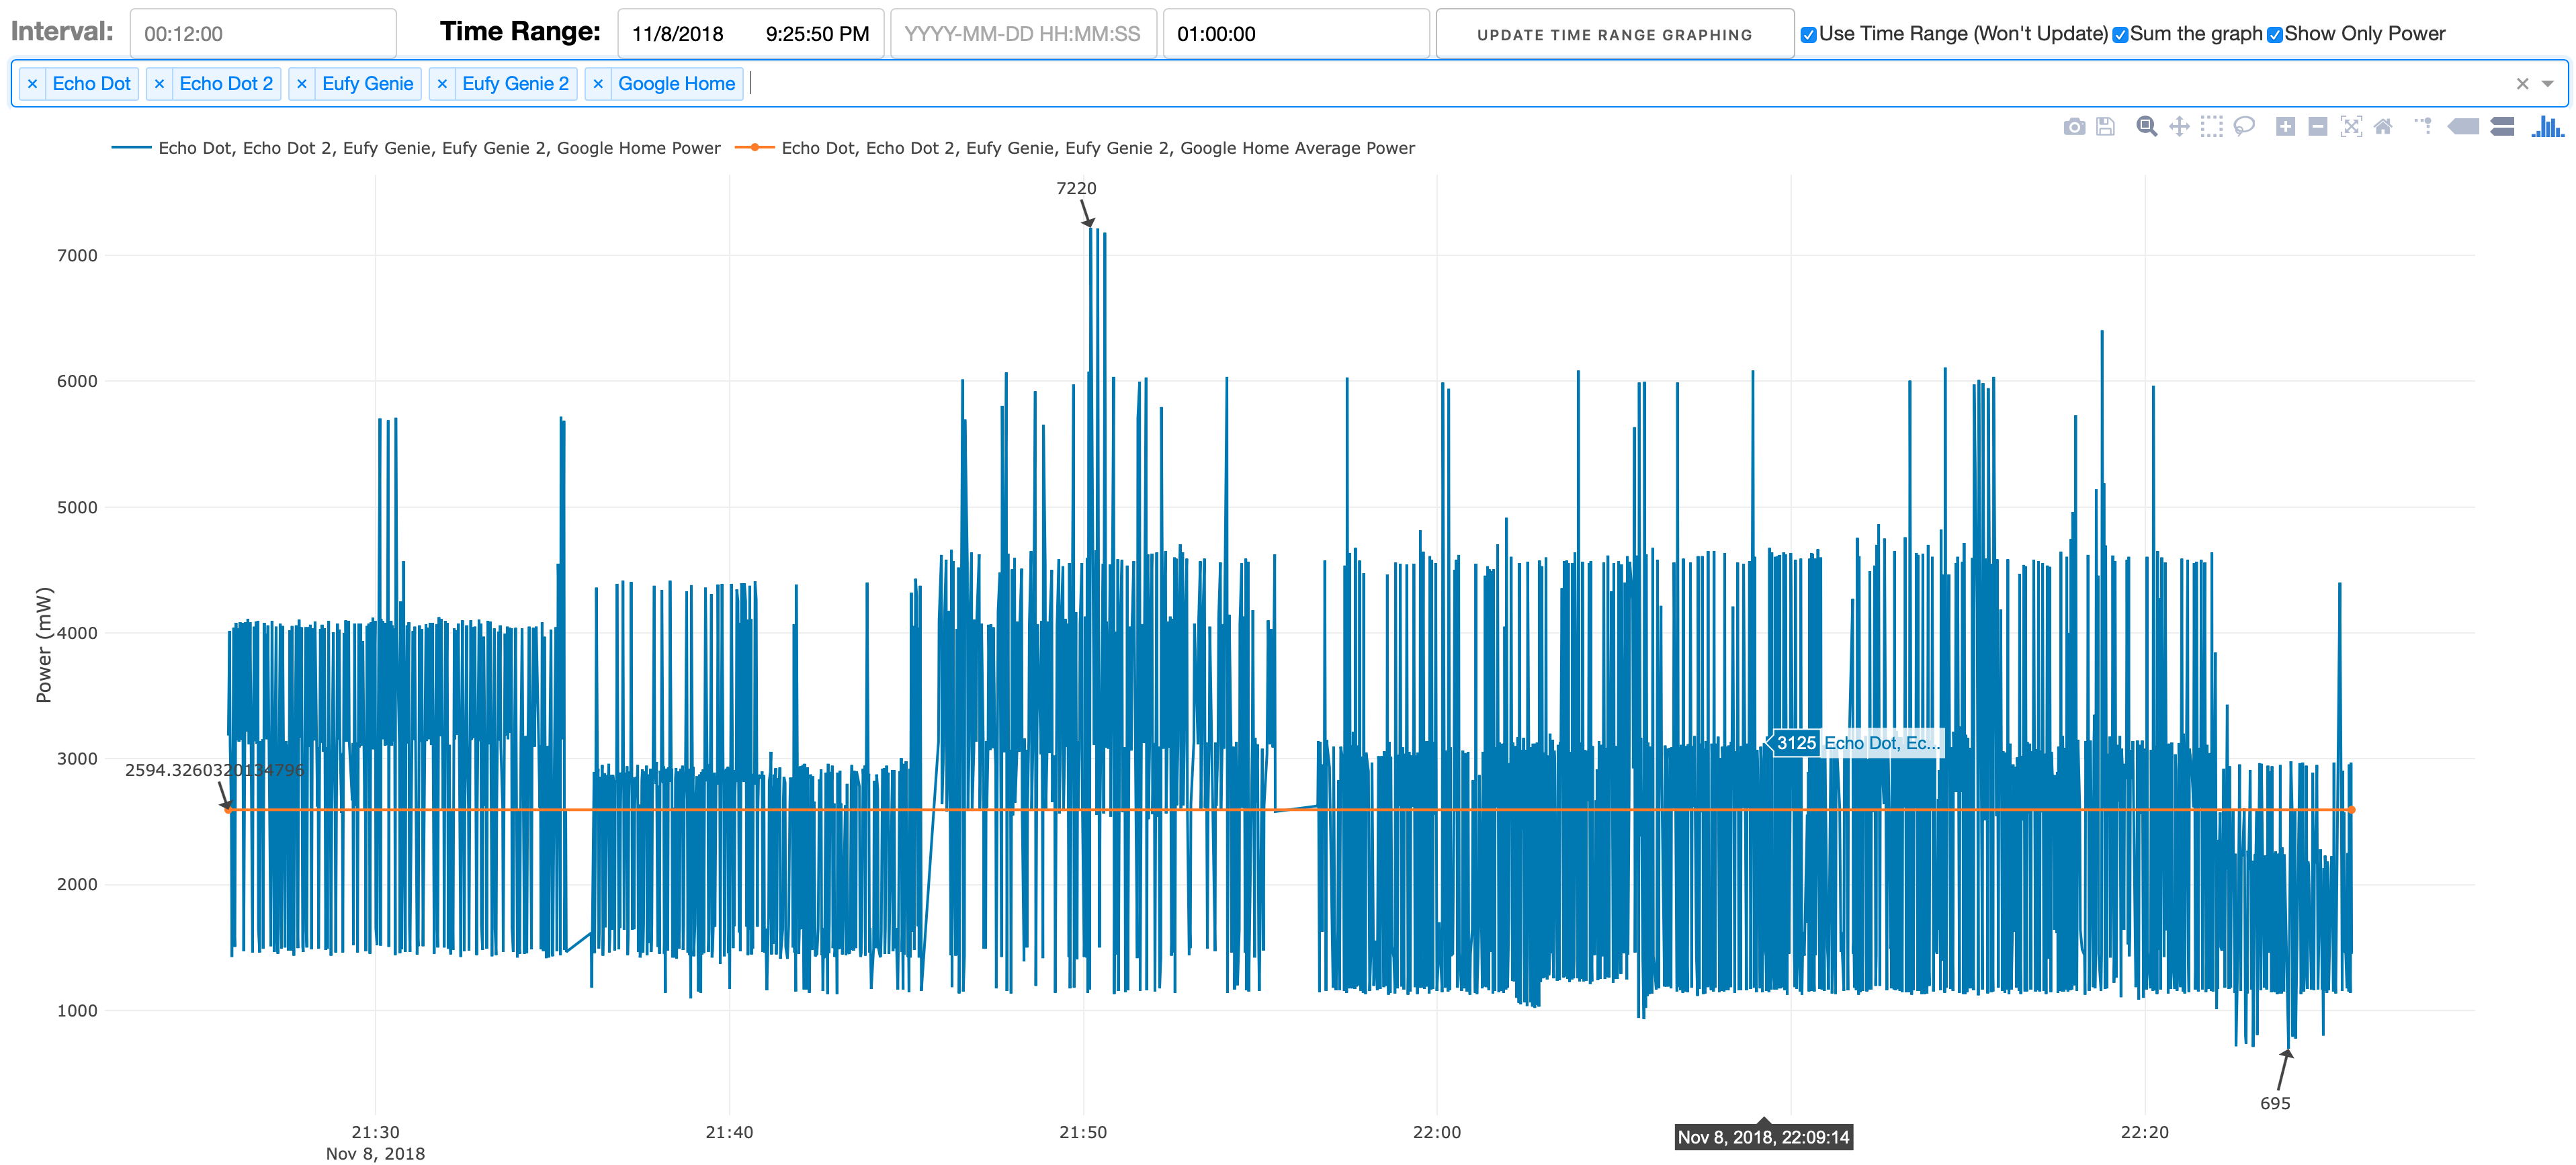
\includegraphics[width=1\textwidth]{figures/noninterpolated.png}
    \caption{Summed power traces without interpolation.}
    \label{fig:noninterpolated}
\end{figure}

\begin{figure}[H]
    \centering
    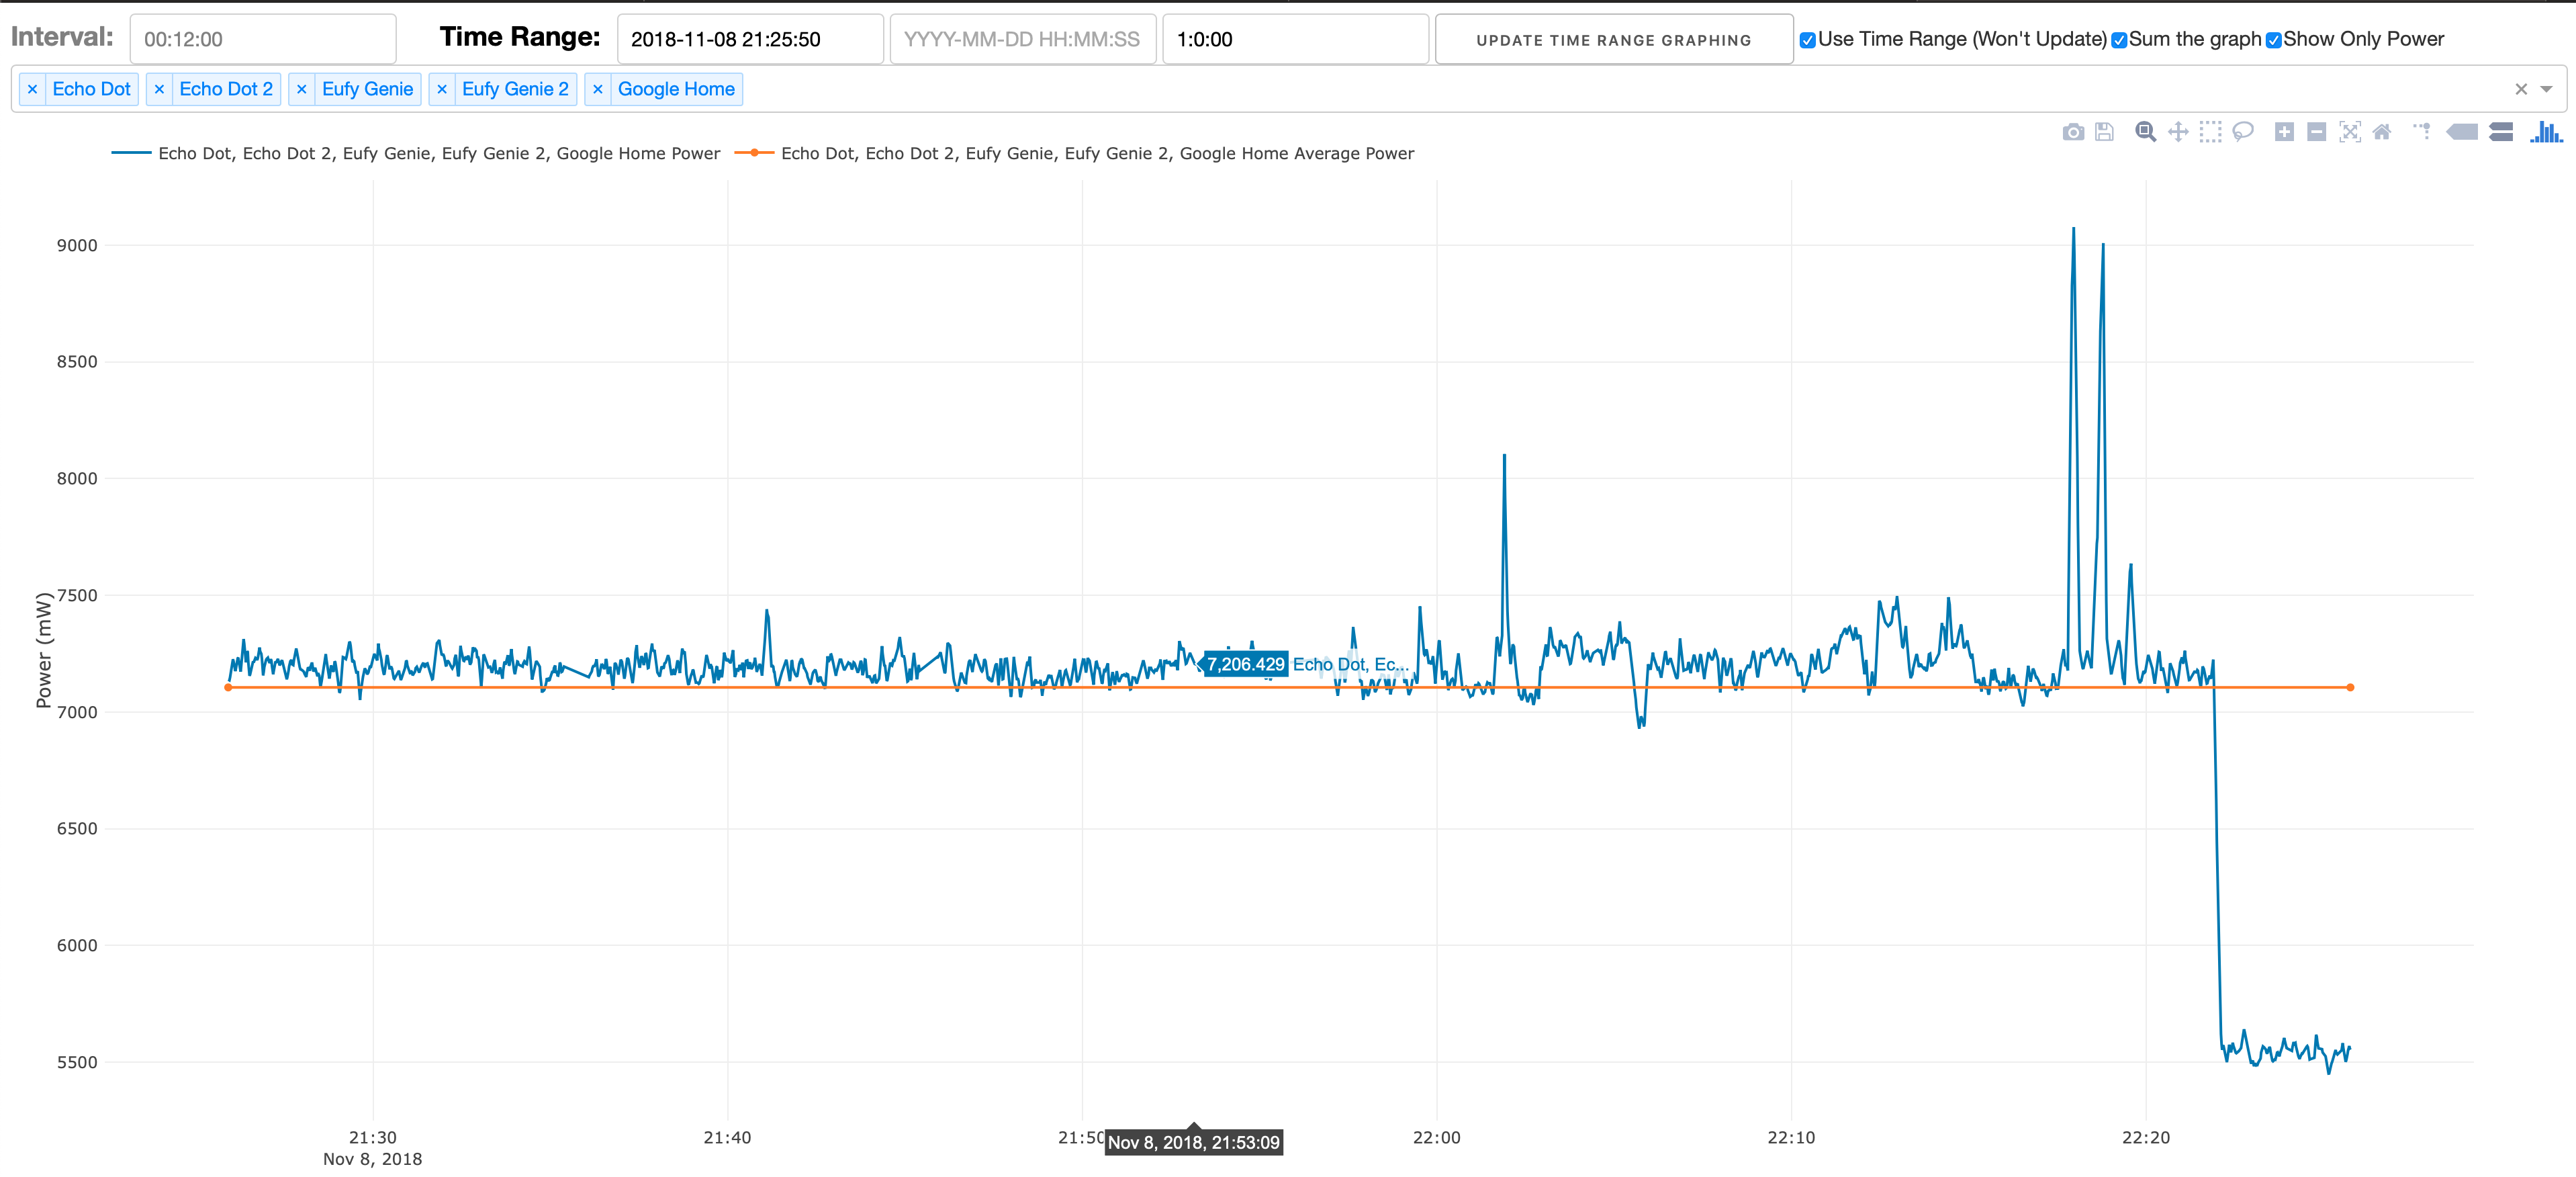
\includegraphics[width=1\textwidth]{figures/interpolated.png}
    \caption{Summed power traces with interpolation.}
    \label{fig:interpolated}
\end{figure}

The grapher can also sum up all power traces into one single trace. Originally, when summing the graphs, it would add the two Pandas \cite{pandas} data frames that represent each trace, and graph the result, shown in figure \ref{fig:noninterpolated}. Pandas is a Python library that represents a multidimensional array as a table, providing useful methods for manipulating the dataset. However, the Wemo doesn't always sample every second. This is an issue if, at time, one device X has a power point, but another device does not. The summation will count the empty data point as 0, resulting in an erroneous sum. This was solved by interpolating data for every second for each device before summing data frames, with a builtin Pandas feature. Interpolation is shown in \ref{fig:interpolated} as a graph.

\subsubsection{Visual Takeaway}
This tool created most of the images shown in section \ref{Results}. A few other researchers such as Frawley's have used this tool for data visualization. The grapher provides real-time or historical graphs on any in the database device for individual analysis or comparison with little effort or time. Additional features from Plotly also provides an easy way to format graphs for presentations or papers.

The summation feature can simplify the graph and provide a more holistic view of power usage, making it easier to spot patterns. In this paper, the summation feature is used to simulate the concept of a household's ``powerline'' where all energy usage would be summed up into one power meter.

\subsubsection{Limitations}
As this tool was created entirely for research purposes, there are some edge cases that it fails to handle.

When the database has too many connections, the software will refuse to connect, and the grapher will not work. When graphing in real time, the grapher makes a new connection for each query. If a query fails, connections can quickly build up.

The graphing tool also slows as the time frame requested increases. We have noticed a slow down for queries with time frames longer than seven hours. In the static graphing mode, the tool slows down before graphing the information. However, in real time graphing mode, the tool will make many slow queries, eventually causing too many connections to the database and undefined behavior.

The graphing tool uses a lookup table that maps the IP address of the device to the corresponding name given to the Wemos. Because we manually create the lookup table, when any of these fields change, the graphing is not able to find the device. In some cases, this causes the graphing tool to crash. To solve this, the user must manually change the IP addresses defined in the lookup table in lines 23-39 shown in listing \ref{lst:ipLookup} below.

To figure out the new IP address for the table, the user must perform a SQL query in the time frame that a particular device is doing something, and manually examine the network traffic to see which IP has the highest network throughput. With this method, we had to ensure only one device was in use so that an IP address for another device would not be confused for the current device.

\begin{minipage}{\textwidth}
    \begin{lstlisting}[label={lst:ipLookup},caption={IP lookup table in real time iot grapher.}]
    #region IP Addresses of all devices we are tracking
    ip = {
        'Chromecast':       '192.168.12.77',
        'Echo Dot 2':       '10.42.0.132',
        'Echo Dot':         '10.42.0.150',
        'Eufy Genie':       '10.42.0.223',
        'Eufy Genie 2':     '10.42.0.172',
        'Fire Stick':       '192.168.12.113',
        'Google Home':      '10.42.0.236',
        'IP Camera':        '192.168.12.58',
        'Nintendo Switch':  '192.168.12.160',
        'Roku':             '192.168.12.68',
        'Samsung Hub':      '192.168.12.100',
        'Samsung TV':       '192.168.12.191',
        'Smart Light':      '192.168.12.27',
        'Xbox':             '192.168.12.251',
        'Echo Show':        '192.168.12.122',
        'Appliance':        '192.168.12.122',
        'Appliance1':        '192.168.12.122',
    }
    \end{lstlisting}
\end{minipage}
